\documentclass{article}
\usepackage{graphicx} % Required for inserting images
\usepackage[utf8]{inputenc}
\usepackage{graphicx}
\usepackage[margin=2.5cm]{geometry}
\usepackage{amssymb}
\usepackage{amsmath}
\usepackage{physics}
\usepackage{bbold}
\usepackage{ragged2e}
\usepackage{setspace}
\usepackage{hyperref}

\setstretch{1.2}
\justifying
\title{Quantum Mechanics 2}
\author{Teo Jin Kiat Joel}
\date{1 September 2023}

\begin{document}

\maketitle

\begin{flushleft}

\hypersetup{}
\tableofcontents

\pagebreak
\section{Introduction}
In this document, Quantum Mechanics will be discussed as followed in PC3130 Quantum Mechanics II, taught by Associate Professor Quek Su Ying. The topics covered will be exactly that as in the module stated above. Namely, Commuting Operators, Symmetries in QM, Angular Momentum Operator, Spin, Identical Particles, Time-independent Perturbation, Time-dependent Perturbation, Variational Principle, Scattering.

\section{Quantum Mechanics Preliminaries}
First, we will have a quick review of the preliminaries of Quantum Mechanics.\\

\subsection{Postulates of Quantum Mechanics}
1. A state of a quantum system is completely specified by $\ket{\psi}$, which propogates in space and time according to the Schrodinger's equation.\\

\smallskip
2. All observables of a quantum system can be described by \textbf{hermitian} operators; measures only the eigenvalues $\lambda$ given the eigenstate $\ket{\Lambda}$.\\

\smallskip
3. The \textbf{probability} of measuring $\lambda$ for $\ket{\psi}$ is given by $\abs{\bra{\Lambda}\ket{\psi}}^2$

\subsection{Basis vectors}
Basis=\{$\ket{\phi_1},\ket{\phi_2},\ket{\phi_3},...\ket{\phi_N}$\}\\

The number of basis vectors equal to the dimension of the Hilbert space in which the quantum states live in. Note that the basis vectors are all normalised. The properties of basis vectors are as follows:\\[0.5cm]

1. Basis vectors are orthonormal: $\bra{\phi_n}\ket{\phi_m}=\delta_{nm}$\\

\smallskip
2. Basis vectors are complete: $\sum_{i=1}^{N}\ket{\phi_i}\bra{\phi_i}=\mathbb{1}$\\[0.5cm]

These mean that any state that exist in the Hilbert space can be expanded as $\sum_{i=1}^{N}\ket{\phi_i}\bra{\phi_i}\ket{\psi}$. There is also a \textbf{linear superposition} of the basis vectors.

\subsection{Observables}
Observables are described by hermitian operators. This is because the nature of hermitian operators is such that the \textbf{eigenvalues} associated with the eigenstates of hermitian operators are always \textbf{real}. Hence, they have a \textbf{physical interpretation} to them.\\

$$\hat{A}\ket{\alpha}=a\ket{\alpha}$$\\

Where $\hat{A}$ is the hermitian operator, $\ket{\alpha}$ is the eigenstate of $\hat{A}$ and $a$ is the eigenvalue(measured value of observable). $\hat{A}$ is hermitian if it is equal to its \textbf{adjoint}. Note that the adjoint of an operator acts on the bra while the operator itself acts on the ket. However, this is a trivial point when dealing with hermitian operators as the adjoint is equal to itself.\\[0.5cm]

If $\hat{A}$ is hermitian,
$$\hat{A}\ket{\psi_1}=\alpha_1\ket{\psi_1}$$
$$\hat{A}\ket{\psi_2}=\alpha_2\ket{\psi_2}$$
$$\alpha_1\neq\alpha_2\rightarrow\bra{\psi_1}\ket{\psi_2}=0$$\\

Eigenstates of hermitian operators that correspond to different eigenvalues are orthonormal. If all eigenvalues are \textbf{distinct}, then the set of eigenstates \textbf{form an orthonormal basis}. This is the case where there is \textbf{no degenderacy}. However, if there is degeneracy, where $\alpha_1=\alpha_2$ and $\ket{\psi_1}\neq\ket{\psi_2}$, there exist a \textbf{linear combination} of $\ket{\psi_1}$ and $\ket{\psi_2}$ that is orthonormal. Thus, there is \textbf{always an orthonormal basis} that diagonalises $\hat{A}$.\\[0.5cm]

In order to measure the \textbf{probability} of the quantum system having a quantum number associated with the observable, the following calculation can be carried out:\\
$$O=\sum_n\lambda_n^{(O)}P_n^{(O)}$$
$$P_n^{(O)}=\sum_i\ket{\Lambda_n^{(O)}}\bra{\Lambda_n^{(O)}}$$
$$This\ is\ the \ spectral\ decomposition\ of\ O$$
$$\mathbb{P}(O=\lambda_n^{(O)})=\bra\psi P_n^{(O)} \ket\psi$$\\

In words, this is the probability of finding the quantum numbers of the observable equal to a particular eigenvalue of the observable when the system is measured.\\[0.5cm]

Lastly, the \textbf{expectation values} of an observable with respect to a quantum state can be calculated. This can be done by considering the action of the hermitian operator on the quantum system.

$$\left\langle\hat{A}\right\rangle_\psi=\bra\psi\hat{A}\ket\psi$$\\
Showing that the expectation value will always be real:\\
$$\left\langle\hat{A}\right\rangle_\psi=\sum_i\alpha_1\abs{c_i}^2$$
$$\abs{c_i}^2\in\mathbb{R}$$\\

The expectation value of an observable can be thought of as the \textbf{mean value} of all the outcomes of the experiment. It is not the probability of attaining a specific outcome, but the average of all the possible outcomes if the experiment is repeated on multiple identical systems.
\pagebreak



\section{Commuting Operators}
\subsection{Commutator and Properties}
Now, we will shift our attention to operators which commute with each other. The mathematical definition of such a property is as follows:

$$[\hat{A},\hat{B}]\equiv\hat{A}\hat{B}-\hat{B}\hat{A}$$
$$\text{For\ commuting\ operators,}$$
$$[\hat{A},\hat{B}]=0$$
$$\therefore\hat{A}\hat{B}-\hat{B}\hat{A}=0$$
    
This is one simple way in which operators are shown to be commuting; they are called \textbf{commutators}. Now, if $[\hat{A},\hat{B}]=0$, then $\hat{A}\hat{B}\ket\psi=\hat{B}\hat{A}\ket\psi$ for all $\ket\psi$. This mean that it does not matter which operator acts on the state first and this is a result of the commutation relationship. Below is a list of \textbf{properties of commutators}:

\begin{align*}
    [\hat{A},\hat{B}]&=-[\hat{B},\hat{A}]\\
    [\hat{A},a]&=0\\
    [\hat{A},a\hat{B}]&=a[\hat{A},\hat{B}]=[a\hat{A},\hat{B}]\\
    [\hat{A},f(\hat{A})]&=0\\
    [\hat{A}\hat{B},\hat{C}]&=[\hat{A},\hat{C}]\hat{B}+\hat{A}[\hat{B},\hat{C}]\\
    [\hat{A},\hat{B}\hat{C}]&=[\hat{A},\hat{B}]\hat{C}+\hat{B}[\hat{A},\hat{C}]\\
    [\hat{A},\Vec{B}\cdot\Vec{C}]&=[\hat{A},\vec{B}]\cdot\Vec{C}+\vec{B}\cdot[\hat{A},\vec{C}]
\end{align*}


Going back to commutators, if $[\hat{A},\hat{B}]=0$,  then $\hat{A}\ and\ \hat{B}$ have a set of \textbf{common eigenstate}. Below is the proof for this claim:\\

\begin{align*}
    \hat{A}\ket{\psi_a}=&a\ket{\psi_a}\\
    \hat{B}\hat{A}\ket{\psi_a}=&\hat{B}a\ket{\psi_a}\\
    \because [\hat{A},\hat{B}]=&0,\\
    \hat{B}\hat{A}\ket{\psi_a}=&\hat{A}\hat{B}\ket{\psi_a}\\
    =&a\hat{B}\ket{\psi_a}\\
    \therefore \hat{B}\ket{\psi_a} \text{is an eigenstate of}\ \hat{A}
\end{align*}

Case 1:\\
If $\ket{\psi_a}$ is the only linearly independent eigenstate of $\hat{A}$ with eigenvalue $a$, then $\hat{B}\ket{\psi_a}$ must be $\mu\ket{\psi_a}$, where $\mu$ is a global pahse. So, $\ket{\psi_a}$ is also an eigenstate of $\hat{B}$.(Recall that eigenstates of an operator do not transform under its own action)\\
\pagebreak

Case 2:\\
If $\ket{\psi_a}$ is not the only linearly independent eigenstate of $\hat{A}$, the system has degeneracies. A degenerate subspace have different eigenstates with the same eigenvalues.\\

$$\hat{A}\ket{\psi_a^{(1)}}=a\ket{\psi_a^{(1)}}$$
$$\hat{A}\ket{\psi_a^{(2)}}=a\ket{\psi_a^{(2)}}$$
$$\ket{\psi_a^{(1)}}\neq\ket{\psi_a^{(2)}}$$

Then, any $\ket{\psi_a}=\alpha\ket{\psi_a^{(1)}}+\beta\ket{\psi_a^{(2)}}$ satisfy $\hat{A}\ket{\psi_a}=a\ket{\psi_a}$. Thus, $\hat{B}\ket{\psi_a}=\alpha'\ket{\psi_a^{(1)}}+\beta'\ket{\psi_a^{(2)}}$. This mean that if $[\hat{A},\hat{B}]=0$ and $a$ is a degenerate eigenvalue of $\hat{A}$, then the corresponding eigenstates of $\hat{A}\ and\ \hat{B}$\textbf{ need not be the same}.\\[0.5cm]

In summary, \textbf{commutators} are important as operators with this property are shown to have the \textbf{same eigenstates if not degenerate}. Going back to the idea of \textbf{observables}, it is convenient to measure a quantum system using commuting observables as it yields ``good quantum numbers" which will be discussed further in the next topic. In addition, commuting observables allow for \textbf{simultaneous measurements} on the subspaces, thus, they are crucial to making useful \textbf{physical interpretation} of the system.

\subsection{Non-commuting Observables}

Are there any use for operators which do not commute? As stated above, commuting observables allow for simultaneous measurements on the subspaces. However, when observables are \textbf{non-commuting}, a problem arises and the system no longer allows for simultaneous measurements. In fact, one important principle is based off the fact that two very important operators in the Hilbert space do not commute.  These operators are the \textbf{position} and \textbf{momentum} operators. Below is the derivation of the commutator relationship between these two operators which yields an interesting yet crucial result in quantum mechanics, the \textbf{Uncertainty Principle}.\\

\begin{align*}
&\hat{X}=\int dx'x'\ket{x'}\bra{x'}\\
\hat{X}&\ket x=x\ket x\\
\hat{P}&\ket{\psi}=\int dx \bigg(-i\hbar \frac{d}{dx}\psi(x)\bigg)\ket x\\
\bra{x}[\hat{X},\hat{P}]&\ket\psi=\hat{X}\hat{P}\psi(x)-\hat{P}\hat{X}\psi(x)\\
\bra{x}[\hat{X},\hat{P}]&\ket\psi=x\bigg(-i\hbar\frac{d}{dx}\psi(x)\bigg)-\bigg(-i\hbar\frac{d}{dx}x\psi(x)-i\hbar\frac{d}{dx}\psi(x)x\bigg)\\
\bra{x}[\hat{X},\hat{P}]&\ket\psi=i\hbar\frac{d}{dx}\psi(x)\\
\therefore[\hat{X}&,\hat{P}]=i\hbar\frac{d}{dx}\mathbb{1}
\end{align*}

This result is known as the  \textbf{Canonical Commutation Relation}. As can be seen, position and momentum do not commute with each other in quantum systems, giving rise to an uncertainty relation between the two operators as follows:
$$\Delta\hat{X}\Delta\hat{P}\geq\frac{\hbar}{2}$$

Hence, position and momentum of a quantum system cannot be measured simultaneously due to this intrinsic uncertainty of the observables.\\[0.5cm]

\subsection{Complete Set of Commuting Observables}

\textbf{Definition} of a complete set of commuting observables(\textbf{CSCO}):\\
An exhaustive set of commuting operators whose common eigenstates are uniquely determined by the eigenvalues of these operators.\\[0.5cm]

Having covered the idea of commuting observables, we are interested in finding a set of commuting observables which is said to be \textbf{complete}. This is because the eigenvalues of the particle's hamiltonian is often \textbf{degenerate}, \textbf{not} allowing one to \textbf{uniquely determine} the state of the system. The way to rectify this issue is to find a complete set of commuting observables which describes the system. For example, if $\hat{A}$ has degenerate eigenvalue $a$, measuring $a$ will not give a unique state. However, if a commuting observable $\hat{B}$ is found to be \textbf{compatible} with $\hat{A}$ with eigenvalue $b$, measuring both $\hat{A}$ and $\hat{B}$ \textbf{simultanously} could yield the result that the system is in the state $\ket{\psi_{ab}}$, which is a \textbf{common eigenstate} of both $\hat{A}$ and $\hat{B}$. Note that the common eigenstate $\ket{\psi_{ab}}$ is a subset of the degenerate eigenstates if $\hat{A}$.\\[0.5cm]

If the eigenvalue of $\hat{A}$ is \textbf{not doubly degenerate}, but have multiple degeneracies, more of such commuting observables can be found such that there is a common eigenstate between all of them which can uniquely determine the state of the system. i.e. $\ket{\psi_{ab...n}}$\\[0.5cm]

Now, measuring an eigenvalue $a$ of the eigenfunction $\psi_{abc}$(the state is now a function as it lives in a subspace of the functional space known as the Hilbert space) will yield what is known as a `good quantum number'.\\[0.5cm]

\textbf{Definition} of good quantum numbers:\\
An independent set of parameters that may be \textbf{simultaneously specified} and which are \textbf{maximally informative}.

\subsection{Application of CSCO and Born-Oppenheimer Approximation}

Using the case of a Hydrogen atom, we will see how CSCO can be applied, and the Born-Oppenheimer approximation will also be introduced. Now, to find the \textbf{stationary states}, we will need the \textbf{hamiltonian's eigenstates}.

$$\hat{H}=\frac{\hat{P_1}}{2m_1}+\frac{\hat{P_2}}{2m_2}+V(\abs{\vec{r_1}-\vec{r_2}})$$
$$\hat{P_1},m_1\rightarrow \text{Proton}$$
$$\hat{P_2},m_2\rightarrow \text{Electron}$$
$$\abs{\vec{r_1}-\vec{r_2}}\rightarrow \text{Distance between proton and electron}$$

\pagebreak
However, the eigenenergies have \textbf{degeneracies $n^2$}. Thus, in order to have \textbf{maximum information} of the system, the eigenstate $\ket{nlm}$ is used to describe the system. These parameters are manifested as such:\\
$n$ refers to the quantum shells, $l$ refers to the orbitals and $m$ refers to orbital subshells.\\ 

Note that $m$ is a \textbf{normal degeneracy}, which arises from the \textbf{system's symmetry} which will be covered in the next topic.\\[0.5cm]

The eigenenergies of the bound states are found to be:

$$E_n=-\frac{\mu e^4}{2\hbar^2}\frac{1}{n^2}$$
$$n=1,2,...N$$
$$-\frac{\mu e^4}{2\hbar^2}\ \text{is the Rydberg constant}$$

In order to use this equation, the atom is assumed to have the proton exactly as the \textbf{geometrical centre of mass}. This is known as the \textbf{Born-Oppenheimer approximation}. The approximation states that the \textbf{electron motion} and the \textbf{nuclear motion} can be \textbf{separated}. The \textbf{nucleus} can be treated as \textbf{stationary} while solving for the eigenvalues of the electrons. Once done, the eigenvalues of the nucleus can be solved. Lastly, for the hydrogen atom, $\{\hat{H},L^2,L_z\}$ form a complete set of commuting observables.\\[0.5cm]

In summary, this section covers the idea of what a CSCO is, and why it is important to know what forms a CSCO for a particular system. The example of the hydrogen atom is used very informally to show the functions of a CSCO and also to introduce the Born-Oppenheimer approximation. Commuting observables are crucial in measuring and understanding any quantum system, thus, finding a complete set of such commuting observables is definitely useful.
\pagebreak

\section{Symmetries in Quantum Mechanics}

What is symmetry? Symmetry in Physics generally refers to a physical system which remains \textbf{unchanged} under some form of \textbf{transformation}. In this case, symmetry in quantum mechanics can be broken down into three different types of symmetries. \textit{Inversion}, \textit{Translation} and \textit{Rotational} symmetries. In this segment, we will look at the three different types of symmetries and what it means for the quantum system to embody such symmetries.

\subsection{Inversion Symmetry}

To consider inversion symmetry, a spatial inversion of the system is impletmented by a parity operator. Parity is a property of a function. A function is said to have odd parity if :
$$f(-x)=-f(x)$$
and even parity if:
$$f(-x)=f(x)$$
Next, the parity operator is defined as:
$$\hat{\pi}\vec{r}\rightarrow -\vec{r}$$
$$\hat{\pi}\psi(\vec{r})\rightarrow\psi(-\vec{r})$$
Eigenvalues of $\hat{\pi}$:\\
If $\phi(\vec{r})$ is an eigenstate of $\hat{\pi}$, $\hat{\pi}\phi(\vec{r})=\mu\phi(\vec{r})$, where $\mu$ is some scalar. Now:
$$\hat{\pi}^2\phi(\vec{r})=\hat{\pi}\hat{\pi}\phi(\vec{r})=\hat{\pi}(\phi(\vec{-r}))=\phi(\vec{r})$$
From definition of eigenstate:
$$\hat{\pi}\phi(\vec{r})=\mu\phi(\vec{r})$$
$$\therefore \mu=\pm 1$$

Hence, eigenstates of $\hat{\pi}$ obey $\hat{\pi}\phi(\vec{r})=\phi(\vec{-r})=\pm\phi(\vec{r})$, odd and even parity.\\[0.5cm]

What is the implications of a system possessing inversion symmetry?\\
We need to understand how the parity operator transforms operators to understand the implications. Consider an operator $\hat{Q}$ transformed by $\hat{\pi}$ to give an new operator $\hat{Q}'$. $\hat{Q}'$ gives the same expectation values in the untransformed state $\ket{\psi}$ as $\hat{Q}$ would give in the transformed state $\ket{\hat{\pi}\psi}$. Mathematically, this means:
$$\bra{\psi}\hat{Q}'\ket{\psi}=\bra{\hat{\pi}\psi}\hat{Q}\ket{\hat{\pi}\psi}$$
$$\bra{\hat{\pi}\psi}\hat{Q}\ket{\hat{\pi}\psi}=\bra{\psi}\pi^\dagger\hat{Q}\pi\ket{\psi}$$
$$\therefore \hat{Q}'=\pi^\dagger\hat{Q}\hat{\pi}$$

If the Hamiltonian of the system $\hat{H}'=\pi^\dagger\hat{Q}\hat{\pi}$, and $[\hat{\pi},\hat{H}]=0$, then there exists a set of common eigenstates between $\hat{\pi}$ and $\hat{H}$. There exists a set of eigenstates of the hamiltonian that have definite parity and are either odd or even. If the eigenstates are non-degenerate, they must have \textbf{definite parity}. This means that $\mu$ is a\textbf{ good quantum number} and \textbf{parity is conserved}.
\pagebreak
\subsection{Translational Symmetry}

Translation is due to the action of a translation operator. It can be visualised as a translation of an arbitrary function.

\begin{figure}[h]
    \centering
    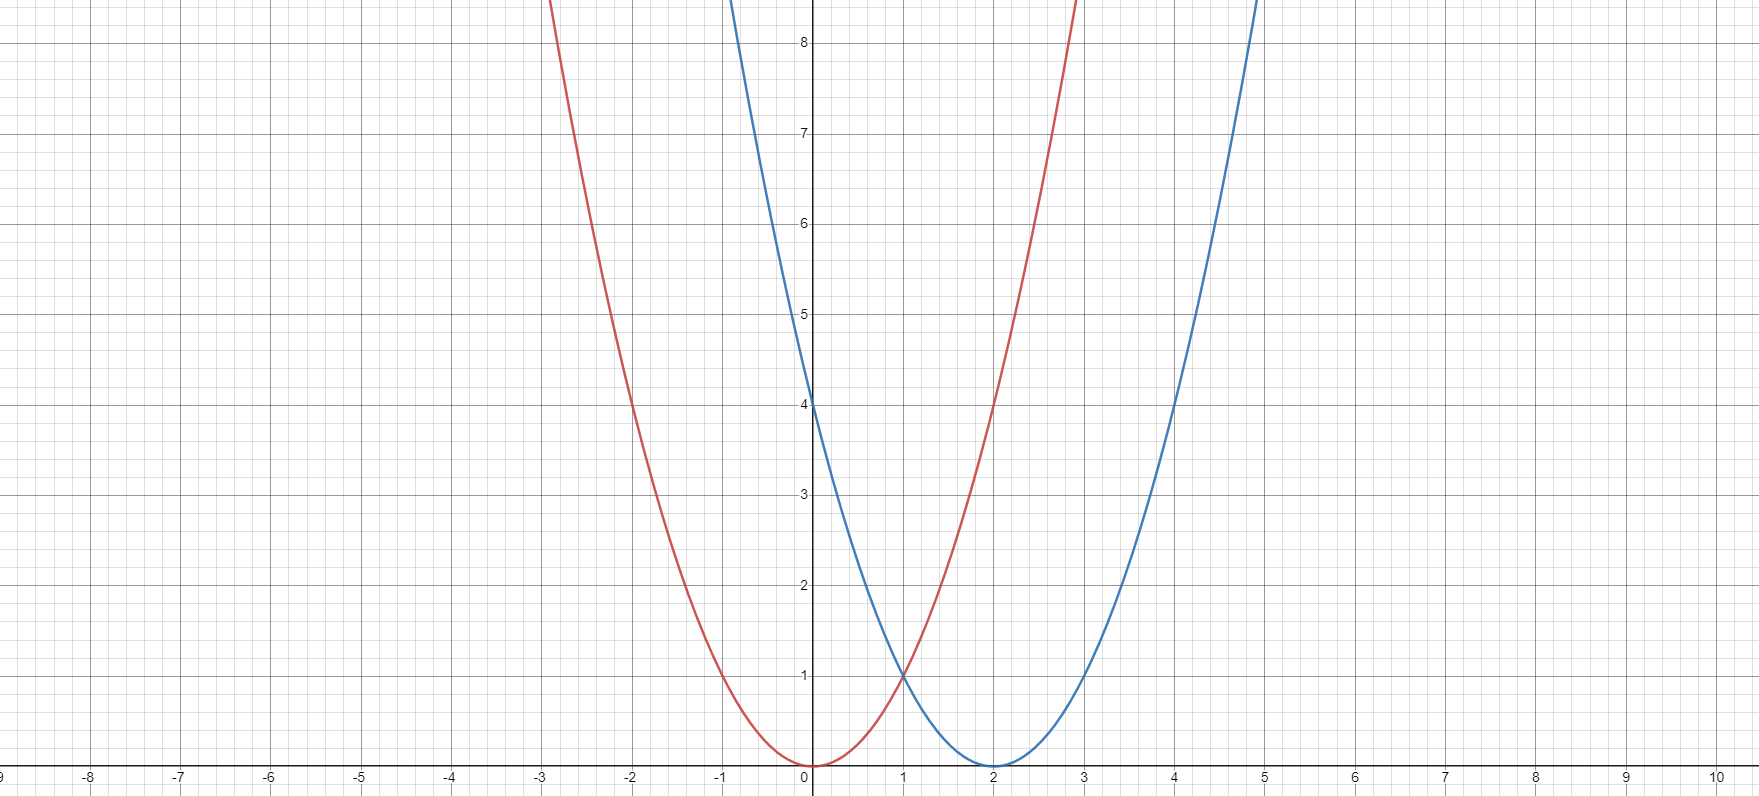
\includegraphics[width=0.8\textwidth]{Capture 1.png}
    \caption{Translation of $y=x^2$ to $y=(x-2)^2$}
    \label{fig:my_label}
    \end{figure}

This action is as shown below:
$$\hat{T}(a)\psi(x)=\psi'(x)=\psi(x-a)$$
Upon expanding the last term by its Taylor's Series, we attain:
$$\hat{T}=e^{-\frac{ia}{\hbar}{\hat{P}}}$$

Note that momentum is the generator of translations.(Read up on group theory for more detail)\\[0.5cm]

If a system has continuous \textbf{translational symmetry}, the \textbf{hamiltonian} is \textbf{invariant under translations}. Also, the momentum operator is conserved. This is congruent with the fact that linear momentum is the generator of translations. Below is the proof:

\begin{align*}
    U^\dagger_\tau H U_\tau&=H\\
    U_\tau U^\dagger_\tau H U_\tau&=U_\tau H\\ 
    \because   U_\tau U^\dagger_\tau&=\mathbb{1}\\
    \therefore HU_\tau&=U_\tau H\\
    [H,U_\tau]&=0\\
    U_\tau&=e^{-\frac{i}{\hbar}\hat{a}\cdot\hat{p}}\\
    \text{for}\ |a|&=da<<1\\
    \text{Taylor's expansion of U:}\\
    U_\tau&\approx 1-i\frac{i}{h}\hat{p}\\
    \therefore [\hat{H},1-i\frac{i}{h}\hat{p}]&=0\\
    [\hat{H},\hat{p}]&=0
    \end{align*}

\subsection{Rotational Symmetry}

The last symmetry to be considered is \textbf{Rotational Symmetry}. Just as how linear momentum is the generator of translations, angular momentum is the generator of rotations. Rotation operators can act on both scalar operators and vector operators. However, by definition, \textbf{scalar} operators do \textbf{not transform under rotations}. This leaves us with the consideration of \textbf{vector operators}, which \textbf{transforms} as a\textbf{ vector under rotations}. The \textbf{expectation} value of a vector operator in the \textbf{rotated state} is obtained by \textbf{rotating} the \textbf{expectation} of the operator in the \textbf{original state}. Below is an example of such a rotation:

\begin{figure}[h]
    \centering
    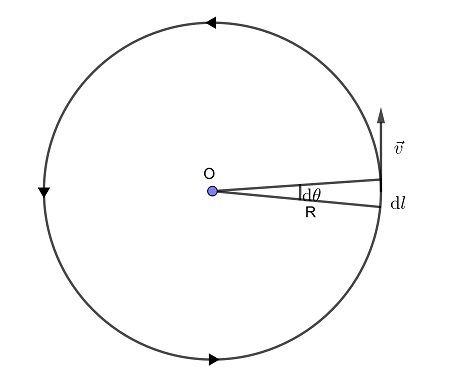
\includegraphics[width=0.35\textwidth]{circle.jpg}
    \caption{Infinitesimal change in angular displacement}
    \end{figure}

$$dl=d\theta(\hat{n}\times\vec{r})$$
$$r'=\vec{r}+d\theta(\hat{n}\times\vec{r})$$
$\hat{A}$ transforms as:
\begin{align*}
\bra{\psi'}\hat{A}\ket{\psi'}&=\bra{\psi}\hat{A}\ket{\psi}+d\theta(\hat{n}\times\bra{\psi}\hat{A}\ket{\psi})\\
\because \psi'&=U_R\psi\\
\therefore LHS&=\bra{\psi}U^\dagger_R\hat{A}U_R\ket{\psi}\\
&=RHS\\
U_R&=e^{-\frac{i}{\hbar}d\theta\hat{n}\cdot\vec{J}}\\
\therefore U^\dagger_R\hat{A}U_R&=(1+\frac{i}{\hbar}d\theta\hat{n}\cdot\vec{J})\hat{A}(1-\frac{i}{\hbar}d\theta\hat{n}\cdot\vec{J})\\
&=\hat{A}+d\theta\frac{i}{\hbar}[\hat{n}\cdot\vec{J},\hat{A}]
\end{align*}
Comparing to RHS:
$$\frac{i}{\hbar}[\hat{n}\cdot\vec{J},\hat{A}]=\hat{n}\times\hat{A}$$
$$[\hat{A},\hat{n}\cdot\hat{J}]=i\hbar(\hat{n}\times\hat{A})$$
$$\rightarrow \text{Definition of vector operator}\ \hat{A}$$

What is the consequence of rotational invariance? For a central potential, the \textbf{hamiltonian commutes} with all components of the \textbf{angular momentum}. Hence, \textbf{angular momentum conservation} is a \textbf{consequence of rotational invariance}. This gives rise to a \textbf{complete} set of commuting observables ${\hat{H},L^2,L_z}$ as seen in chapter 3.
\pagebreak

\section{Angular Momentum}
\subsection{Ladder Operators}
In this chapter, we will analyse the eigenstates and eigenvalues of the angular momentum operator of a quantum system. The approach that will be used is to apply an angular momentum ladder operator onto the eigenstates of the angular momentum. In order to understand this, a recap of how ladder operators has to be done. Hence, we shall see how the ladder operators function in a 1-dimensional harmonic oscillator.

\begin{align*}
    a^\dagger&=\sqrt{\frac{m\omega}{2\hbar}}\hat{X}-\frac{i}{\sqrt{2m\hbar\omega}}\hat{P} &
    a&=\sqrt{\frac{m\omega}{2\hbar}}\hat{X}+\frac{i}{\sqrt{2m\hbar\omega}}\hat{P}\\[0.5cm]
    &\textbf{Properties:}\\
\end{align*}
\begin{align}
    [a,a^\dagger]&=\mathbb{1}\\
    N&\equiv \ a^\dagger a\\
    [N,a]&=-a\\
    [N,a^\dagger]&=a^\dagger
\end{align}
You may convice yourself that these relations are true by using the relations (1) and (2) to derive the rest.\\
Note that $a^\dagger$ is the \textbf{raising operator} which promotes an eigenstate to the next quantized level, while $a$ is the \textbf{annihilation operator} which demotes an eigenstate to the previous quantized level. At the ground state of the harmonic oscillator, the annihilation operator does not further demote the state.\\[0.5cm]
Now, taking $\ket{n}$ to be the  eigenstate of the harmonic oscillator, the action of the ladder operators are as such:
$$a\ket{n}=\sqrt{n}\ket{n-1}$$
$$a^\dagger\ket{n}=\sqrt{n+1}\ket{n+1}$$
Eg.
\begin{align*}
\bra{n-2}a^2\ket{n}&=\bra{n-2}aa\ket{n}\\
&=a^\dagger\bra{n-2}(a\ket{n})\\
&=\sqrt{n-1}\bra{n-1}\sqrt{n}\ket{n-1}\\
&=\sqrt{n(n-1)}
    \end{align*}

The eigenenergies of the corresponding energy eigenstates are given by the following relation:
$$E_n=\bigg(n+\frac{1}{2}\bigg)\hbar\omega$$
Hence, it can be seen that for a 1-dimensional harmonic oscillator, the ladder operators provide an easy way to find the eigenenergies. Similarly, we can find the angular momentum eigenvalues of a quantum system by using appropriate ladder operators.

First, the angular momentum operator follows these two commutation relations:
$$[J_i,J_j]=i\hbar\epsilon_{ijk}J_k$$
$$[J^2,J_i]=0$$
The proof for the first relation is as follows, considering only orbital angular momentum:
\begin{align*}
    [r_i,p_j]&=i\hbar\delta_{ij}\\
    \vec{L}&=\vec{r}\times \vec{p}\\
    [L_i,L_j]&=\epsilon_{mni}r_mp_n\epsilon_{abj}r_ap_b-\epsilon_{abj}r_ap_b\epsilon_{mni}r_mp_n\\
    &=[\epsilon_{mni}r_mp_n,\epsilon_{abj}r_ap_b]\\
    &=\epsilon_{mni}\epsilon_{abj}[r_,p_n,r_a,p_b]\\
    &=\epsilon_{mni}\epsilon_{abj}([r_mp_n,r_a]p_b+r_a[r_mp_n,p_b])\\
    &=\epsilon_{mni}\epsilon_{abj}(-[r_a,p_n]r_m+[r_m,p_b]p_n)\\
    &=\epsilon_{mni}\epsilon_{abj}(-i\hbar\delta_{an}r_mp_b+i\hbar\delta_{mb}p_nr_a)\\
    &=i\hbar\epsilon_{mni}\epsilon_{abj}\delta_{mb}p_nr_a-i\hbar\epsilon_{mni}\epsilon_{abj}\delta_{an}r_mp_b\\
    &=i\hbar\epsilon_{abj}(\epsilon_{bni}p_nr_a-\epsilon_{mai}r_mp_b)\\
    &=i\hbar(\epsilon_{bja}\epsilon_{bni}p_nr_a-\epsilon_{abj}\epsilon_{aim}r_mp_b)\\
    &=i\hbar[(\delta_{jn}\delta_{ai}-\delta_{ji}\delta_{an}p_nr_a)-(\delta_{bi}\delta_{jm}-\delta_{bm}\delta_{ji}r_mp_b)]\\
    &=i\hbar[p_jr_i-p_ar_a\delta_{ji}-(r_jp_i-r_bp_b\delta_{ij})]\\
    &=i\hbar(r_ip_j-r_jp_i)\\
    \therefore [L_i,L_j]&=i\hbar\epsilon_{ijk}L_k
\end{align*}
This is a very general proof in any 3-dimensional right-handed orthogonal system. Now, a proof in the cartesian basis can be done for the second commutation relation as follows:
\begin{align*}
    [L^2,L_z]&=[L_x^2,L_z]+[L_y^2,L_z]+[L_z^2,L_z]\\
    &=[L_xL_x,L_z]+[L_yL_y,L_z]+[L_zL_z,L_z]\\
    \text{Using}\ [AB,C]&=[A,C]B+A[B,C]\\
    &=[L_x,L_z]L_x+L_x[L_x,L_z]+[L_y,L_z]L_y+L_y[L_y,L_z]\\
    &=-i\hbar L_yL_x-i\hbar L_xL_y+i\hbar L_yL_x+i\hbar L_xL_y\\
    &=0
\end{align*}
In this case, $J=L$ as only orbital angular momentum is considered. However, this relation can be generalised to incorporate spin angular momentum.\\

Coming back to the idea of the ladder operator; since $J^2$ and $J_i$ commutes, there exists a set of \textbf{common eigenstates} between them. The ladder operator to be found will then either promote or demote the eigenstate to the adjacent eigenstates. The corresponding raising and lowering operators are below:
$$J_+=J_x+iJ_y$$
$$J_-=J_x-iJ_y$$
The eigenstate of this system is $\ket{j,m}$ where:
$$J^2\ket{j,m}=\hbar^2j(j+1)\ket{j,m}$$
$$J_z\ket{j,m}=m\hbar\ket{j,m}$$
$$-j\le m\le j,\ m=-j,-j+1,...j-1,j$$

It is useful to consider the \textbf{matrix representation} of the ladder operators. Hence, below is an example of how to form the matrix representation of a half-spin system:
$$J_\pm\ket{j,m}=\hbar\sqrt{j(j+1)-m(m\pm1)}\ket{j,m\pm1}$$
$$\text{Eigenbasis:}\ \ket{s,m}$$
$$s=\frac{1}{2}$$
$$m=-\frac{1}{2},\frac{1}{2}$$
$$Let\ \ket{s=\frac{1}{2},m=-\frac{1}{2}}=\begin{pmatrix}
    0\\1
    \end{pmatrix},$$
$$\ket{s=\frac{1}{2},m=\frac{1}{2}}=\begin{pmatrix}
    1\\0
    \end{pmatrix}$$
$$\therefore S_+\ket{s,.m-\frac{1}{2}}=\hbar\ket{s,m=\frac{1}{2}},$$
$$S_-\ket{s,.m-\frac{1}{2}}=\hbar\ket{s,m=-\frac{1}{2}}$$
Applying $J_+$ on $\ket{s,m=-\frac{1}{2}}$ state, we will get $\hbar\ket{s,m=\frac{1}{2}}$.
Thus, $J_+$ must be:
$$
\begin{pmatrix}
    a&b\\
    c&d
\end{pmatrix}\begin{pmatrix}
    0\\1
\end{pmatrix}
=\hbar
\begin{pmatrix}
  1\\0  
\end{pmatrix}$$
$$\therefore J_+=
\begin{pmatrix}
    0&\hbar\\
    0&0
\end{pmatrix}$$
Similarly, $J_-$ can be found the same way, and will be:
$$J_-=\begin{pmatrix}
    0&0\\
    \hbar&0
\end{pmatrix}$$

Now, after finding the matrix representations of the ladder operators, the other angular momentum operators $J_x$ and $J_y$ can be found by the relation below:
$$J_\pm=J_x\pm iJ_y$$
$$\therefore J_x=\frac{1}{2}(J_++J_-),$$
$$J_y=\frac{1}{2i}(J_+-J_-)$$
Practically, one can check if their matrix representations of the angular momentum operators are accurate by checking against the first commutation relation in page 12. Hence, having found $J_x$ and $J_y$ using the ladder operators, one can compute $[J_x,J_y]\overset{!}{=} i\hbar\epsilon_{xyz}J_z$.\\[0.5cm]
Topic not discussed: \textbf{Eigenfunctions}. The eigenfunctions of $L^2$ and $L_z$ are the spherical harmonics, for more information, refer to Griffiths.
\pagebreak

\subsection{Addition of Angular Momentum}
\subsubsection{Spin}
\textbf{Spin} in classical mechanics can be thought of as the angular momentum of a body rotating about a fixed axis with respect to the axis. In quantum mechanics, it is not quite so simple. Spin in quantum mechanics refers to an \textbf{intrinsic property} of the particle. For example, an electron has a spin $s=\frac{1}{2}$, even though the electron is not literally a ball rotating about some axis. Spin in quantum mechanics, unlike its classical analogue, is \textbf{not geometrical}.\\[0.5cm]

Notice that in the previous example, we used spin as the example for formulating the angular momentum ladder operators. It holds as \textbf{spinor algebra} is the same as the algebra used in analysing orbital angular momentum. To better understand spinors, we will need the notion of \textbf{tensor products}, which will be covered in the next chapter.\\[0.5cm]

Coming back to the spin-half system, we can carry on from the previous example to work out what $J_x$ and $J_y$ actually are. Below is the working:

\begin{align*}
J_x&=\frac{1}{2}(J_++J_-)\\
&=\begin{pmatrix}
    0&\frac{\hbar}{2}\\
    0&0
\end{pmatrix}
+
\begin{pmatrix}
    0&0\\
    \frac{\hbar}{2}&0
\end{pmatrix}\\
&= \begin{pmatrix}
    0&\frac{\hbar}{2}\\
    \frac{\hbar}{2}&0
\end{pmatrix}\\
&=\frac{\hbar}{2}
\begin{pmatrix}
0&1\\
1&0    
\end{pmatrix}
\end{align*}

\begin{align*}
J_y&=\frac{1}{2i}(J_+-J_-)\\
&=\begin{pmatrix}
    0&\frac{\hbar}{2i}\\
    0&0
\end{pmatrix}
-
\begin{pmatrix}
    0&0\\
    \frac{\hbar}{2i}&0
\end{pmatrix}\\
&= \begin{pmatrix}
    0&\frac{\hbar}{2i}\\
    \frac{-\hbar}{2i}&0
\end{pmatrix}\\
&=\frac{\hbar}{2}
\begin{pmatrix}
0&-i\\
i&0    
\end{pmatrix}
\end{align*}

Notice that these are exactly the two Pauli spin matrices. Also, using the same eigenbasis, $J_z$ is as follows($J_z$ is \textbf{diagonalised} with \textbf{eigenvalues} $m\hbar$ as the eigenstates are eigenbasis of this operator):
$$J_z=\frac{\hbar}{2}
\begin{pmatrix}
    1&0\\
    0&-1
\end{pmatrix}$$
Therefore we attain the three \textbf{Pauli spin operators} weighted by $\frac{\hbar}{2}$:
$$\sigma_x=
\begin{pmatrix}
0&1\\
1&0    
\end{pmatrix},
\sigma_y=
\begin{pmatrix}
0&-i\\
i&0    
\end{pmatrix},
\sigma_z=
\begin{pmatrix}
    1&0\\
    0&-1
\end{pmatrix}$$

\subsubsection{Tensor Product}

When considering the new angular momentum of two quantum systems, a composite state is to be found in a tensor product space. Given vector spaces $\nu_1$ and $\nu_2$, we can define a tensor product space:
$$\nu\equiv\nu_1\otimes\nu_2$$
Given that the basis vectors of $\nu_1$ and $\nu_2$ are $\{\ket{u_i(1)}\}$ and $\{\ket{u_j(2)}\}$ respectively, the new basis of $\nu$ are $\{\ket{u_i(1)}\otimes\ket{u_j(2)}\}$. In the same way, for every vector $\ket{\psi(1)}$ belonging to $\nu_1$ and $\ket{\phi(2)}$ belonging to $\nu_2$, there exists a vector $\ket{\psi(1)}\otimes\ket{\phi(2)}$. Eg:
$$\nu_1=\{e_1,e_2\},$$
$$\nu_2=\{g_1,g_2\}$$
$$\nu\equiv\nu_1\otimes\nu_2$$
$$\nu=\{e_1g_1,e_1g_2,e_2g_1,e_2g_2\}$$

\textbf{Properties} of tensor product space:\\[0.5cm]
1.) Linearity
$$(\lambda\ket{\psi(1)})\otimes\ket{\phi(2)}=\lambda(\ket{\psi(1)}\otimes\ket{\phi(2)})$$
$$\ket{\psi(1)}\otimes(\ket{\phi_1(2)}+\ket{\phi_2(2)})=\ket{\psi(1)}\otimes\ket{\phi_1(2)}+\ket{\psi(1)}\otimes\ket{\phi_2(2)}$$
Note that not all vectors in the new tensor product space can be written in the form $\ket{\psi(1)}\otimes\ket{\phi(2)}$; such states are \textbf{entangled}. For a two level system, these are the \textbf{Bell states}.\\[0.2cm]

Tensor product of \textbf{operators}:
$$(\hat{A}(1)\otimes\hat{B}(2))(\ket{\psi(1)}\otimes\ket{\phi(2)})=\hat{A}(1)\ket{\psi(1)}\otimes\hat{B}(2)\ket{\phi(2)}$$
Essentially what is happening is the operator only acts on the state which belongs to its own vector space.\\[0.5cm]
2.) Product
$$(\hat{A}(1)\otimes\hat{B}(2))(\hat{A}(1)'\otimes\hat{B}(2)')=(\hat{A}(1)\hat{A}(1)')\otimes(\hat{B}(2)\hat{B}(2)')$$\\[0.5cm]

3.) Trace
$$Tr(\hat{A}(1)\otimes\hat{B}(2))=Tr(\hat{A}(1))-Tr(\hat{B}(2))$$\\[0.5cm]

4.) Adjoint
$$(\hat{A}(1)\otimes\hat{B}(2))^\dagger\ket{\psi(\nu)}=\hat{A}(1)^\dagger\otimes\hat{B}(2)^\dagger\ket{\psi(\nu)}$$\\[0.5cm]

5.) Dimension
$$\nu_1\rightarrow n_1$$
$$\nu_2\rightarrow n_2$$
$$\nu\rightarrow n_1n_2$$
Eg. Dimension
$$\vec{s}=\{-1,0,1\},\ \vec{L}=\{l_1,l_2\}$$
$$\vec{J}=\vec{s}+\vec{L}$$
$$D_s=3,\ D_L=2$$
$$\therefore D_J=6$$

Eg. Action
\begin{align*}
    \vec{s}(\ket{\psi}\otimes\ket{\phi})&=(\vec{s}\otimes\mathbb{1})(\ket{\psi}\otimes\ket{\phi})\\
    &=(\vec{s}\ket{\psi})\otimes(\mathbb{1}\ket{\phi})\\
    &=\vec{s}\ket{\psi}\otimes\ket{\phi}\ (\text{Similarly for}\ \vec{L})\\
    \vec{J}(\ket{\psi}\otimes\ket{\phi})&=(\vec{s}\otimes\mathbb{1}+\mathbb{1}\otimes\vec{L})(\ket{\psi}\otimes\ket{\phi})\\
    &=(\vec{s}\ket{\psi}\otimes\ket{\phi})+(\ket{\psi}\otimes\vec{L}\ket{\phi})\\
    \end{align*}
Therefore $\vec{J}$ acts on the new tensor product space.\\[.5cm]
Tensor product \textbf{matrix representation}:
\begin{align*}
a&=\begin{pmatrix}
   a_1&a_2\\
   a_3&a_4
\end{pmatrix}\quad
b=\begin{pmatrix}
    b_1&b_2\\
    b_3&b_4
\end{pmatrix}\\
a\otimes b&=\begin{pmatrix}
    a_1\begin{pmatrix}
    b_1&b_2\\
    b_3&b_4
\end{pmatrix}&a_2\begin{pmatrix}
    b_1&b_2\\
    b_3&b_4
\end{pmatrix}\\
a_3\begin{pmatrix}
    b_1&b_2\\
    b_3&b_4
\end{pmatrix}&a_4\begin{pmatrix}
    b_1&b_2\\
    b_3&b_4
\end{pmatrix}
\end{pmatrix}
\end{align*}
\begin{align*}
    \sigma^x_1\otimes\sigma^x_2&=\begin{pmatrix}
        0&1\\
        1&0
    \end{pmatrix}\otimes\begin{pmatrix}
        0&1\\
        1&0
    \end{pmatrix}\\
    &=\begin{pmatrix}
        0\begin{pmatrix}
        0&1\\
        1&0
    \end{pmatrix}&1\begin{pmatrix}
        0&1\\
        1&0
    \end{pmatrix}\\
    1\begin{pmatrix}
        0&1\\
        1&0
    \end{pmatrix}&0\begin{pmatrix}
        0&1\\
        1&0
    \end{pmatrix}
    \end{pmatrix}\\
    &=\begin{pmatrix}
        0&0&0&1\\
        0&0&1&0\\
        0&1&0&0\\
        1&0&0&0
    \end{pmatrix}
\end{align*}

\subsubsection{Representations}

Suppose an angular momentum $\hat{J}(1)$ acts in the space $\nu_1$ and $\hat{J}(2)$ acts on the state $\nu_2$, then there exists a new angular momentum:
$$\hat{J}=\hat{J}(1)\otimes\mathbb{1}(1)+\mathbb{1}(2)\otimes\hat{J}(2)$$
which acts on $\nu_1\otimes\nu_2$. What are the possible values of $m$ and $j$ for the new $\hat{J}$? Recall:
$$\hat{J}^2\ket{j,m}=\hbar^2j(j+1)\ket{j,m}$$
$$\hat{J_z}\ket{j,m}=m\hbar\ket{j,m}$$
Thus, two quantum numbers were required to completely describe the eigenstates in $\nu_1$ and $\nu_2$ each. Now, how many \textbf{quantum numbers} are required to describe the new eigenstates in $\nu_1\otimes\nu_2$?
$$\ket{j_1,m_1}\otimes\ket{j_2,m_2}\in\nu_1\otimes\nu_2$$
$$\{\ket{j_1,m_1}\otimes\ket{j_2,m_2};m_1=-j_1,j_1+1,...,j_1,m_2=-j_2,-j_2+1,...,j_2\}$$
$$\text{Dimension of}\ \nu_1\otimes\nu_2=(2j_1+1)(2j_2+1)$$
Hence, the new space requires \textbf{four} quantum numbers $(j_1,m_1,j_2,m_2)$ to \textbf{fully specify} the eigenstates $\ket{j_1,m_1,j_2,m_2}$. This is known as the \textbf{uncoupled representation}.\\[0.5cm]

Next, we will look at the \textbf{coupled representation}. In order to specify the eigenstates in the new tensor product space, there has to be four quantum numbers. From the original vector spaces, there are only two good quantum numbers. Hence, two more need to be found. This can be done by finding operators which commute with $\hat{J}^2$ and $\hat{J_z}$. Possible candidates include $\hat{J_1}^2,\hat{J_2}^2,\hat{J_{1z}},\hat{J_{2z}}$.
\begin{align*}
    [\hat{J}^2,\hat{J_1}^2]&=[\hat{J_1}^2+\hat{J_2}^2+2\hat{J_1}\hat{J_2},\hat{J_1}^2]\\
    &=[\hat{J_1}^2,\hat{J_1}^2]+[\hat{J_2}^2,\hat{J_1}^2]+[2\hat{J_1}\hat{J_2},\hat{J_1}^2]\\
    &=[2\hat{J_1}\hat{J_2},\hat{J_1}^2]\\
    &=2([\hat{J_1},\hat{J_1}^2]\hat{J_2}+\hat{J_1}[\hat{J_2},\hat{J_1}^2])\\
    &=0
\end{align*}
* Note that commutators from different spaces commute, and commutators commute with itself.\\
The same result can be obtained for $[\hat{J}^2,\hat{J_2}^2]$. Now, looking at commutators with $\hat{J_z}$:
\begin{align*}
   [\hat{J_z},\hat{J_1}^2]&=[\hat{J_{1z}}+\hat{J_{2z}},\hat{J_1}^2]\\
   &=0
\end{align*}
Once again, the same result can be obtained for $[\hat{J_z},\hat{J_2}^2]$. Therefore, $\{\hat{J}^2,\hat{J_z},\hat{J_1}^2,\hat{J_2}^2\}$ is a set of \textbf{mutually commuting observables} in $\nu_1\otimes\nu_2$. Their eigenstates can be specified as $\ket{j,m,j_1,j_2}$ with four good quantum numbers $j,m,j_1,j_2$.\\[0.5cm]

When is it more convenient to use the coupled representation? When a system has \textbf{internal} interactions, it is more convenient to use the \textbf{coupled} representation. On the other hand, when a multiparticle system only interacts with an \textbf{external} field or source, it is more convenient to use the \textbf{uncoupled} representation.\\
Eg. Hamiltonian interacting with external field:
$$\hat{H}=\hat{H_1}+\hat{H_2}$$
$$\{\hat{H},\hat{s}_{1z},\hat{s}^2_1,\hat{s}_{2z},\hat{s}^2_2\}\ \text{forms a CSCO} $$
Eg. 2 spins interacting with each other:
$$\hat{H}=\alpha\hat{s_1}\cdot\hat{s_2}$$
\begin{align*}
    [\hat{H},\hat{s}_{1z}]&=[\alpha(\hat{s}_{1x}\hat{s}_{2x}+\hat{s}_{1y}\hat{s}_{2y}+\hat{s}_{1z}\hat{s}_{2z}),\hat{s}_{1z}]\\
    &=\alpha([\hat{s}_{1x},\hat{s}_{1z}]\hat{s}_{2x}+[\hat{s}_{1y},\hat{s}_{1z}]\hat{s}_{2y}+[\hat{s}_{1z},\hat{s}_{1z}]\hat{s}_{2z})\\
    &=\alpha i\hbar(\hat{s}_{1x}\hat{s}_{2x}-\hat{s}_{1y}\hat{s}_{2x})\\
    &\neq 0
\end{align*}
Thus, $m_1$ and $m_2$ are not good quantum numbers for the second system. Therefore, the \textbf{coupled representation} would be more apt for this system.\\[0.5cm]

Next, to find the values which the new $j$ can take, use the \textbf{Triangulation Rule} as follows:
$$\hat{J}=\hat{j_1}+\hat{j_2}$$
$$m=m_1+m_2$$
$$j_{max}=j_1+j_2$$
$$j_{min}=\abs{j_1-j_2}$$
$$j=j_{min},j_{min}+1,...,j_{max}-1,j_{max}$$

Now, we will look at how one can switch between coupled and uncoupled representations. The system to be considered will be the total spin angular momentum of \textbf{two spin-half} particles. Start off by listing out all the possible eigenstates of the new angular momentum space in both uncoupled and coupled representation. Then, using ladder operators, find the coefficients of the coupled eigenstates. Do the same for the uncoupled eigenstates. Lastly, compare to find the coefficients when converting from coupled to uncoupled
representation. These coefficients are called the\textbf{ Clebsch-Gordon coefficients}.

$$S_1=\frac{1}{2},\ \ S_2=\frac{1}{2}$$
$$m_1=-\frac{1}{2},\frac{1}{2}\ \ m_2=-\frac{1}{2},\frac{1}{2}$$
$$\text{Dimension:}\ 2(j+1)=4$$
$$S=S_1+S_2=0,1$$
Possible eigenstates(uncoupled representation):
\begin{align*}
    m=1&\rightarrow\ket{m_1=\frac{1}{2},m_2=\frac{1}{2}}\\
    m=0&\rightarrow\ket{m_1=\frac{1}{2},m_2=-\frac{1}{2}},\ket{m_1=-\frac{1}{2},m_2=\frac{1}{2}}\\
    m=-1&\rightarrow\ket{m_1=-\frac{1}{2},m_2=-\frac{1}{2}}
\end{align*}
Possible eigenstates(coupled representation):
\begin{align*}
    m=1&\rightarrow\ket{s=1,m=1}\\
    m=0&\rightarrow\ket{s=1,m=0},\ket{s=0,m=0}\\
    m=-1&\rightarrow\ket{s=1,m=-1}
\end{align*}
Now, using ladder operators in the coupled representation:
\begin{align*}
    S_+\ket{s=1,m=-1}&=\hbar\sqrt{s(s+1)-m(m+1)}\ket{s=1,m=0}\\
    &=\sqrt{2}\hbar\ket{s=1,m=0}
\end{align*}
Doing the same for the uncoupled representation:
\begin{align*}
    (S_{1+}+S_{2+})\ket{m_1=-\frac{1}{2},m_2=-\frac{1}{2}}&=[(S_{1+}\otimes\mathbb{1})+(\mathbb{1}\otimes S_{2+})]\bigg(\ket{m_1=-\frac{1}{2}}\otimes\ket{m_2=-\frac{1}{2}}\bigg)\\
    &=\hbar\sqrt{s_1(s_1+1)-m_1(m_1+1)}\ket{m_1=\frac{1}{2}}\otimes\ket{m_2=-\frac{1}{2}}\\
    &+\hbar\sqrt{s_2(s_2+1)-m_2(m_2+1)}\ket{m_1=-\frac{1}{2}}\otimes\ket{m_2=\frac{1}{2}}
\end{align*}
Comparing the coupled and uncoupled representations, we get:
$$\ket{s=1,m=0}=\frac{1}{\sqrt{2}}\bigg(\ket{m_1=\frac{1}{2},m_2=-\frac{1}{2}}+\ket{m_1=-\frac{1}{2},m_2=\frac{1}{2}}\bigg)$$
Hence, this is the Clebsch-Gordon coefficients with respect to the coupled representation $\ket{s=1,m=0}$. Remember that for the $m=0$ configuration, there should be a second coupled eigenstate $\ket{s=0,m=0}$. However, since the ladder operators that are used on the coupled representation eigenstates hold \textbf{$s$ as a fixed value}, it is not possible to attain the second set of Clebsch-Gordon coefficients.\\[0.5cm]

In order to find the second set of coefficients which corresponds to the $\ket{s=0,m=0}$ eigenstate, the \textbf{orthogonality} of the states can be used. Since the eigenstates are orthogonal, the inner product between them is $0$.
$$\braket{s=1,m=0}{s=0,m=0}=0$$
Allowing $\ket{s=0,m=0}$ to have arbitrary coefficients in the uncoupled representation $a$ and $b$ to be solved:
$$\frac{1}{\sqrt{2}}\bigg(\bra{m_1=\frac{1}{2},m_2=-\frac{1}{2}}+\bra{m_1=-\frac{1}{2},m_2=\frac{1}{2}}\bigg)\bigg(a\ket{m_1=\frac{1}{2},m_2=-\frac{1}{2}}+b\ket{m_1=-\frac{1}{2},m_2=\frac{1}{2}}\bigg)=0$$
$$\therefore a=-b=\frac{1}{\sqrt{2}}$$
$$\therefore \ket{s=0,m=0}=\frac{1}{\sqrt{2}}\bigg(\ket{m_1=\frac{1}{2},m_2=-\frac{1}{2}}-\ket{m_1=-\frac{1}{2},m_2=\frac{1}{2}}\bigg)$$
Thus, the coefficients found are:
$$\frac{1}{\sqrt{2}},\frac{1}{\sqrt{2}},\frac{1}{\sqrt{2}},-\frac{1}{\sqrt{2}}$$
Note that for this method to work, if the coupled eigenstate is being \textbf{raised}, the uncoupled eigenstate must also be \textbf{raised} so that the yielded coefficients will align accordingly. Finally, one may wonder about the states where $m=1$ and $m=-1$. The short answer to that would be that the coupled and uncoupled representation of those eigenstates have a 1 to 1 mapping. Hence, the Clebsch-Gordon coefficients for those states will be 1. To be sure, one can check if that is true using the same method. 

Below is the table comparing the coupled and uncoupled representations of this system.


\begin{table}[h]
        \centering
    \begin{tabular}{|c|c|c|}
    \hline
        \multicolumn{2}{|c|}{Coupled} &Uncoupled \\
        \hline
         s&  m& $m=\frac{1}{2}\equiv\uparrow,m=-\frac{1}{2}\equiv\downarrow$\\
         \hline
         1&  1& $\ket{\uparrow\uparrow}$\\
         \hline
         1&  0& $\frac{1}{\sqrt{2}}(\ket{\uparrow\downarrow}+\ket{\downarrow\uparrow})$\\
         \hline
         1&  -1& $\ket{\downarrow\downarrow}$\\
         \hline
         0&  0& $\frac{1}{\sqrt{2}}(\ket{\uparrow\downarrow}-\ket{\downarrow\uparrow})$\\
         \hline
    \end{tabular}
    \caption{coupled and Uncoupled Representations}
    \label{tab:my_label}
\end{table}
Note that for $s=1$, the system is \textbf{symmetric} with respect to particle exchange, while for $s=0$, the system is \textbf{antisymmetric}. This will be used in the next chapter on identical particles.\\[0.5cm]

As a reminder, this chapter started off with the algebraic analysis of angular momentum using \textbf{ladder operators} that are analogous to the harmonic oscillator. Following that, the idea of \textbf{spin} was discussed, leading up to the derivation of the Pauli matrices. Next, the chapter aimed to cover the \textbf{addition of angular momentum}. An introduction on \textbf{tensor product} was done, explaining that after adding the angular momenta of a system, the new angular momentum lives in a tensor product space, defined by the original vector spaces which the original angular momenta live in. Next, the two different representations, \textbf{coupled and uncoupled representations} of the new angular momentum were discussed. Finally, a practical method to convert between couplings were shown to yield the \textbf{Clebsch-Gordon coefficients}.\\[.5cm]

In the next chapter, we will look at identical and indistinguishable particles in quantum mechanics.
\pagebreak

\section{Indentical and Indistinguishable Particles}

Classically, one can distinguish ``identical"particles by their respective path and velocities. In quantum mechanics, it is not possible to distinguish ``identical" particles because of the \textbf{uncertainty principle}. Examples of ``identical" particles in classical physics would be billiard balls of the same size, mass and color. On the other hand, ``identical" particles in quantum physics could be electrons or protons etc.\\
\textbf{Notation:}
$$\text{Distinguishable}\rightarrow\ \psi(x_1,x_2)=\phi_1(x_1)\chi_2(x_2)$$
$$x_1,x_2\rightarrow \text{Particles}$$
$$\phi,\chi\rightarrow \text{States, Orbits}$$

When two \textbf{identical} particles are being exchanged, the \textbf{observable should not change}. The corresponding wavefunction would either stay the same, or acquire a negative sign, depending the nature of the particle. In the case of \textbf{Bosons}, the wavefunction stays the \textbf{same}, while for \textbf{Fermions}, the wavefunction acquires a\textbf{ negative} sign.\\[.5cm]
\subsection{Bosons, Fermions}
Example: \textbf{Bosons} with possible states $\ket{g}$, $\ket{e}$:
Allowed states:
$$\ket{gg}, \ket{ee}$$
Disallowed states:
$$\ket{ge},\ket{eg}$$
This is because it is \textbf{not possible} to \textbf{distinguish} the configuration of the two states of the combined wavefunction. Hence, another allowed state would be to sum over the possible configurations:
$$\frac{1}{\sqrt{2}}(\ket{ge}+\ket{eg})$$


Example: Fermions, 3 particles, 3 states\\
This can be expressed using Slater determinant. Notice that the sign will flip when a particle is being exchanged.
$$\ket{\Phi}\propto 
\begin{vmatrix}
     \ket{\phi}_{A} & \ket{\phi}_{B} & \ket{\phi}_{C}\\ 
     \ket{\chi}_{A} & \ket{\chi}_{B} & \ket{\chi}_{C}\\
     \ket{w}_{A} & \ket{w}_{B} & \ket{w}_{C} 
\end{vmatrix}$$

\begin{table}[h]
    \centering
    \begin{tabular}{|c|c|c|}
    \hline
       &\textbf{ Boson}    & \textbf{Fermion}\\
         \hline
     Spin  & Integer  & Half-integer \\
         \hline
      Function & Mediate interactions & Constituents of matter\\
      \hline
    Examples &Photon, Phonons, Z, W  & Electron, Neutron, Proton\\
    \hline
      Composite & Even no. of Fermions & Odd no. of Fermions \\
         \hline
        Symmetry & Symmetric & Antisymmetric\\
         \hline
         Statistics & Bose-Einstein & Fermi-Dirac\\
         \hline
        $\ket{\Phi}=\ket{\chi}\otimes\ket{\Psi}$ &If $\ket{\chi}$ is symmetric, $\ket{\Psi}$ also symmetric  & If $\ket{\chi}$ is symmetric, $\ket{\Psi}$ is antisymmetric\\
        \hline
    
    \end{tabular}
    \caption{Boson Vs Fermion}
   \end{table}

\pagebreak

\subsection{Pauli's Exclusion Principle}
Analysing the combined wavefunction of two fermions:
$$\ket{\Phi}=\ket{\phi_1\phi_2}$$
Then:
$$\ket{\Psi}=\frac{1}{\sqrt{2}}(\ket{\uparrow\downarrow}-\ket{\downarrow\uparrow})\otimes\ket{\phi_1\phi_2}$$
Remember that the state $\ket{\phi}$ represents the \textbf{orbit}. Hence, in this example, the two particles are in the \textbf{same orbit}, but have \textbf{opposite spins}. This is because of the property from the table in the previous page. For fermions, when the orbital states are symmetric, the spin states must be antisymmetric. This is also known as the\textbf{ Pauli's Exclusion Principle}. This ensures that the system of electrons in an atom is \textbf{stable}, as no symmetric spin electrons will occupy the same orbit. Since the main interaction between electrons in an atom is \textbf{coulombic} and depends on the square of the \textbf{distance} between electrons, this ensures that the intra-coulombic interactions are \textbf{minimised}.

\pagebreak
\section{Approximation Methods(Time-independent)}
In this chapter, we will learn how to use \textbf{approximation methods} to find the energy eigenstates of time-independent Hamiltonian. THis is because most hamiltonians cannot be solved analytically, but can only be approximated to appropriate degrees. What hamiltonians can be solved? These include the Hydrogen Atom, Infinite Square Well and the Harmonic Oscillator. Examples of approximation methods include the Born-Oppenheimer Approximation, Central Potential and Variational Principle. In this chapter, we will delve deeper into the Variational Principle.\\[.5cm]

\subsection{Variational Principle}
The variational principle can be used to approximate the ground state hamiltonian. This principle ensures that there exist eigenstates of the hamiltonian given by $\hat{H}\ket{\psi_n}=E_n\ket{\psi_n}$. Considering any wavefunction $\ket{\psi}$, one can show that $\bra{\psi}\hat{H}\ket{\psi}\geq E_0$. Below is the proof.

\begin{align*}
    \ket{\psi}&=\sum_n C_n\ket{\psi_n}\\
    \bra{\psi}\hat{H}\ket{\psi}&=\bra{\psi}\hat{H}\sum_n C_n\ket{\psi_n}\\
    &=\sum_n C_n\bra{\psi}E_n\ket{\psi_n}\\
    &=\sum_n C_nE_n\bra{\psi}\ket{\psi_n}\\
    &=\sum_n E_n \abs{C_n}^2\\
    \therefore&\ E_n\geq E_0\ for\ all\ n
\end{align*}
Practically, one can select a \textbf{trial wavefunction} based on well chosen parameters. Minimising $\bra{\psi}\hat{H}\ket{\psi}$ gives the best estimate for $E_0$. The trial wavefunction must be normalised, and must satisfy boundary conditions.\\[.5cm]

The more one \textbf{minimises} the expectation of the hamiltonian, the closer to the groundstate the solution becomes. In order to minimise, the \textbf{space} which is being worked in has to be \textbf{expanded}. The question then becomes: How do we expand the Hilbert space for a better estimate? One way which can be done is to consider \textbf{linear combinations} of different $\Psi$, eg. $\Psi_0+\Psi_1+\Psi_2$ where $\{\Psi_0,\Psi_1,\Psi_2\}$ is an orthogonal basis.\\
Example, hydrogen atom:

Choose spatially symmetric wavefunctions
\begin{align*}
    \Psi_0(\vec{r}_1,\vec{r}_2)&=\frac{1}{\sqrt{2}}(s_1(\vec{r}_1)s_2(\vec{r}_2)+s_2(\vec{r}_1)s_1(\vec{r}_2))\\
    \Psi_1(\vec{r}_1,\vec{r}_2)&=s_1(\vec{r}_1)s_1(\vec{r}_2)\\
    \Psi_2(\vec{r}_1,\vec{r}_2)&=s_2(\vec{r}_1)s_2(\vec{r}_2)\\
    \text{Define}\ \epsilon&=\bra{s_1}H^{sp}\ket{s_1}=\bra{s_2}H^{sp}\ket{s_2}\quad \text{*sp=single particle}\\
    \gamma&=\bra{s_1}\ket{s_2}\approx 0\\
    t&=-\bra{s_1}H^{sp}\ket{s_2}\\
    \Delta&=\bra{\Psi_0}\frac{e^2}{\abs{\vec{r}_1-\vec{r}_2}}\ket{\Psi_0}\\
    \rightarrow Solving\ &for\ \bra{\Psi_0}H^{sp}\ket{\Psi_0}:\\
    \bra{\Psi_0}H_1^{sp}\otimes\mathbb{1}_2\ket{\Psi_0}&=\frac{1}{2}(\bra{s_1}\otimes\bra{s_2}+\bra{s_2}\otimes\bra{s_1})(H_1^{sp}\otimes\mathbb{1}_2)(\ket{s_1}\otimes\ket{s_2}+\ket{s_2}\otimes\ket{s_1})\\
    &=\frac{1}{2}(\bra{s_1}H_1^{sp}\ket{s_1}\bra{s_2}\ket{s_2}+\bra{s_2}H_1^{sp}\ket{s_2}\bra{s_1}\ket{s_1})\\
    \intertext{*Note that the subscript of s denotes the orbital, not the space.}
    &=\frac{1}{2}(\epsilon_1+\epsilon_2)\\
    &=\epsilon\\
    \text{Similarly,}\ \bra{\Psi_0}\mathbb{1_1}\otimes H_2^{sp}\ket{\Psi_0}&=\epsilon\\
    \therefore \bra{\Psi_0}H\ket{\Psi_0}&=2\epsilon+\Delta\\
    \\
    \text{Doing the same for}\ \ket{\Psi_1}\ and\ \ket{\Psi_2}:\\
    \bra{\Psi_1}H\ket{\Psi_1}&=\bra{\Psi_2}H\ket{\Psi_2}=2\epsilon+U\\
    U&=\bra{s_1s_2}\frac{e^2}{\abs{\vec{r}_1-\vec{r}_2}}\ket{s_1s_2}\\
    \text{U represents the on-site repulsion}\\
    U&>\Delta\\
    \because 2\epsilon+\Delta &\geq E_0\\
    \therefore 2\epsilon+U &\geq E_0
    \end{align*}
This brings us to the limitation of this approximation using only one wavefunction. We are unable to get close enough to the groundstate eigenvalue. Hence, to mitigate this issue, a linear combination of wavefunctions can be used.
\pagebreak

\subsection{Non-degenerate Perturbation}
Perturbation is an approximation method used to solve for hamiltonians that are otherwise unsolvable through analytical means. The method requires an \textbf{exact hamiltonian}. Next, a small perturbation is applied to the system, giving a \textbf{series solution} to the new problem. Generally, only perturbations up to the \textbf{second order} are kept as higher order perturbations tend to be negligible. What is the second order perturbation? Looking back at Taylor's expansion:
$$f(x)=f(a)+f'(a)(x-a)+\frac{f''(a)}{2!}(x-a)^2+...$$
This is the Taylor's expansion of $f(x)$ up to the second order. Similarly, perturbation up to this expression will be considered when approximating. Time-independent perturbation takes two forms, \textbf{non-degenerate and degenerate} perturbation theory. As the names suggests, the different methods are used for systems which either have non-degenerate or degenerate eigenstates. In this section, systems of non-degenerate eigenstates will be discussed. Adding a perturbation to an original hamiltonian:
$$H=H_0+\Bar{V}$$
$$\bar{V}=\lambda V$$
$$H_0\ket{\psi_n^0}=E_n^0\ket{\psi_n^0}$$
Where $\bar{V}$ is a small perturbation to the system. The first thing to do is to check if the eigenenergy is degenerate. If not,
\begin{align}
    E_n^1&=\bra{\psi_n^0}\Bar{V}\ket{\psi_n^0}\\
    E_n^2&=\sum_{m\neq n}\frac{\abs{\bra{\psi_m^0}\bar{V}\ket{\psi_n^0}}^2}{E_n^0-E_m^0}\\
    \ket{\psi_n^1}&=\sum_{m\neq n}\frac{\bra{\psi_m^0}\bar{V}\ket{\psi_n^0}}{E_n^0-E_m^0}\ket{\psi_m^0}
\end{align}
Showing equation (5):
\begin{align*}
    \ket{\psi_n}&=\ket{\psi_n^0}+\lambda\ket{\psi_n^1}+\lambda^2\ket{\psi_n^2}+...\\
    E_n&=E_n^0+\lambda E_n^1+\lambda^2 E_n^2+...\\
    \lambda&<<1\\
    \bra{\psi_n^0}\ket{\psi_n^1}&=0\ \text{(Orthogonal)}\\
    \because H\ket{\psi_n}&=E_n\ket{\psi_n}\\
    \therefore (H_0+\lambda V)\ket{\psi_n}&=E_n\ket{\psi_n}\\
    (H_0+\lambda V)(\ket{\psi_n^0}+\lambda\ket{\psi_n^1}+\lambda^2\ket{\psi_n^2})&=(E_n^0+\lambda E_n^1+\lambda^2 E_n^2)(\ket{\psi_n^0}+\lambda\ket{\psi_n^1}+\lambda^2\ket{\psi_n^2})\\
    \end{align*}
Coefficients of $\lambda^0:\ H_0\ket{\psi_n^0}=E_n^0\ket{\psi_n^0}$\\
Coefficients of $\lambda^1:\ H_0\ket{\psi_n^1}+V\ket{\psi_n^0}=E_n^0\ket{\psi_n^1}+E_n^1\ket{\psi_n^0}$\\
\pagebreak
Operating $\bra{\psi_n^0}$ on both sides:

\begin{align*}
    \bra{\psi_n^0}H_0\ket{\psi_n^1}+\bra{\psi_n^0}V\ket{\psi_n^0}&=\bra{\psi_n^0}E_n^0\ket{\psi_n^1}+\bra{\psi_n^0}E_n^1+\ket{\psi_n^0}\\
    \because \bra{\psi_n^0}\ket{\psi_n^1}&=0\\
    E_n^1&=\bra{\psi_n^0}V\ket{\psi_n^0}\text{(shown)}
\end{align*}

Note that first correction of $E_n=\lambda E_n^1=\bra{\psi_n^0}\bar{V}\ket{\psi_n^0}$. Now, showing equation (7):

\begin{align*}
    \sum\ket{\psi_n^0}\bra{\psi_n^0}&=\mathbb{1}\\
    \ket{\psi_n^1}&=\sum_{m\neq n}\ket{\psi_m^0}\bra{\psi_m^0}\ket{\psi_n^1}\\
    \text{Operating}\ \bra{\psi_m^0}\ \text{onto coefficient of}\ \lambda^1:\\
    \bra{\psi_m^0}H_0\ket{\psi_n^1}+\bra{\psi_m^0}V\ket{\psi_n^0}&=\bra{\psi_m^0}E_n^0\ket{\psi_n^1}+\bra{\psi_m^0}E_n^1+\ket{\psi_n^0}\\
    For\ m&\neq n\\
    E_m^0\bra{\psi_m^0}\ket{\psi_n^1}+\bra{\psi_m^0}V\ket{\psi_n^0}&=E_n^0\bra{\psi_m^0}\ket{\psi_n^1}\\
    (E_n^0-E_m^0)\bra{\psi_m^0}\ket{\psi_n^1}&=\bra{\psi_m^0}V\ket{\psi_n^0}\\
    \therefore \ket{\psi_n^1}&=\sum_{m\neq n}\frac{\bra{\psi_m^0}V\ket{\psi_n^0}}{(E_n^0-E_m^0)}\ket{\psi_m^0}\text{(shown)}
\end{align*}

Now, showing equation (6), expanding up to coefficients of $\lambda^2$:

\begin{align*}
    H_0\ket{\psi_n^2}+V\ket{\psi_n^1}&=E_n^0\ket{\psi_n^2}+E_n^1\ket{\psi_n^1}+E_n^2\ket{\psi_n^0}\\
    \text{Operating}\ \bra{\psi_n^0}\ &\text{onto coefficient of}\ \lambda^2:\\
    \bra{\psi_n^0}H_0\ket{\psi_n^2}+\bra{\psi_n^0}V\ket{\psi_n^1}&=\bra{\psi_n^0}E_n^0\ket{\psi_n^2}+\bra{\psi_n^0}E_n^1\ket{\psi_n^1}+\bra{\psi_n^0}E_n^2\ket{\psi_n^0}\\
    E_n^2&=\bra{\psi_n^0}V\ket{\psi_n^1}\\
    &=\bra{\psi_n^0}V\sum_{m\neq n}\frac{\bra{\psi_m^0}V\ket{\psi_n^0}}{(E_n^0-E_m^0)}\ket{\psi_m^0}\\
    &=\sum_{m\neq n}\frac{\abs{\bra{\psi_m^0}V\ket{\psi_n^0}}^2}{(E_n^0-E_m^0)}\text{(shown)}
\end{align*}
Having shown how the eigenenergies appear up to the second correction term, and how the eigenstate of the first correction term looks like, examples using the \textbf{time-independent non-degenerate perturbation} can be explored. In the first example, the system in question is an infinite square well with two bosons.\\
Set-up:
$$\Bar{V}=-aV_0\delta(x_1-x_2)$$
$$\text{Single-particle groundstate}=\sqrt{\frac{2}{a}}sin\frac{\pi x}{a}$$
Solving for the \textbf{first order} correction term of the eigenenergy:
\begin{align*}
    \ket{\psi_1^0(x_1,x_2)}&=\ket{\psi_1^0}\otimes\ket{\psi_1^0}\\
    &=\frac{2}{a}\sin\frac{\pi x_1}{a}\sin\frac{\pi x_2}{a}\\
    E_1^1&=\bra{\psi_1^0}\bar{V}\ket{\psi_1^0}\\
    &=-aV_0\int_0^a dx_1\int_0^a dx_2 \bigg(\frac{2}{a}\bigg)^2\sin^2\frac{\pi x_1}{a}\sin^2\frac{\pi x_2}{a}\delta(x_1-x_2)\\
    &=-aV_0\bigg(\frac{2}{a}\bigg)^2\int_0^a \sin^4\frac{\pi x_1}{a} dx_1\\
    &=-aV_0\bigg(\frac{2}{a}\bigg)^2\int_0^a (\frac{1-\cos\frac{2\pi x}{a}}{2})^2 dx\\
    &=-aV_0\bigg(\frac{1}{a}\bigg)^2\int_0^a (1-2\cos\frac{2\pi x}{a}+\cos^2\frac{2\pi x}{a}) dx\\
    &=-aV_0\bigg(\frac{1}{a}\bigg)^2\int_0^a (1-2\cos\frac{2\pi x}{a}+\frac{1-\cos\frac{4\pi x}{a}}{2}) dx\\
    \because \sin(2\pi)&=0,\\
    \therefore E_1^1&=-aV_0\bigg(\frac{1}{a}\bigg)^2\frac{3}{2}a\\
    &=-\frac{3}{2}V_0
\end{align*}
Note that for functions with \textbf{odd parity}, the expectation value is 0. This can be understood by taking the integral of an odd function about the point of inflexion. In the next example, perturbation of a \textbf{harmonic oscillator} due to an \textbf{electric field} will be studied.\\
Example: Find the first and second order correction terms for a harmonic oscillator perturbed by an external electric field.

\begin{align*}
    H_0&=\frac{p^2}{2m}+\frac{1}{2}m\omega^2x^2 & V&=-qEx
\end{align*}
\begin{align*}
   E_n^0&=(n+\frac{1}{2})\hbar\omega\\
    E_n^1&=\bra{\psi_n^0}V\ket{\psi_n^0}\\
    &=-qE\bra{\psi_n^0}x\ket{\psi_n^0}\\
    &=0\ (\psi_n^0\ \text{is odd about}\ x=0)\\
    E_n^2&=\sum_{m\neq n}\frac{\abs{\bra{\psi_m^0}V\ket{\psi_n^0}}^2}{E_n^0-E_m^0}\\
    \end{align*}
In order to find $\bra{\psi_m^0}V\ket{\psi_n^0}$, use the ladder operators.
\begin{align*}
    a^\dagger&=\sqrt{\frac{m\omega}{2\hbar}}\hat{X}-\frac{i}{\sqrt{2m\hbar\omega}}\hat{P} &
    a&=\sqrt{\frac{m\omega}{2\hbar}}\hat{X}+\frac{i}{\sqrt{2m\hbar\omega}}\hat{P}\\[0.5cm]
\end{align*}

\begin{align*}
    \bra{\psi_m^0}V\ket{\psi_n^0}&=(qE)^2\bra{\psi_m^0}x\ket{\psi_n^0}\\
    x&=(a^\dagger+a)\sqrt{\frac{\hbar}{2m\omega}}\\
    \therefore \bra{\psi_m^0}V\ket{\psi_n^0}&=(qE)^2\bra{\psi_m^0}(a^\dagger+a)\sqrt{\frac{\hbar}{2m\omega}}\ket{\psi_n^0}\\
    &=(qE)^2\sqrt{\frac{\hbar}{2m\omega}}\bra{\psi_m^0}(a^\dagger+a)\ket{\psi_n^0}\\
    &=(qE)^2\sqrt{\frac{\hbar}{2m\omega}}(\bra{\psi_m^0}a^\dagger\ket{\psi_n^0}+(\bra{\psi_m^0}a\ket{\psi_n^0})\\
    &=(qE)^2\sqrt{\frac{\hbar}{2m\omega}}(\sqrt{n}\bra{\psi_m^0}\ket{\psi_{n-1}^0}+\sqrt{n+1}\bra{\psi_m^0}\ket{\psi_{n+1}^0})\\
    &=(qE)^2\sqrt{\frac{\hbar}{2m\omega}}(\sqrt{n}\delta_{m,n-1}+\sqrt{n+1}\delta_{m,n+1})\\
    \therefore E_n^2&=(qE)^2\frac{\hbar}{2m\omega}\sum_{m\neq n}\frac{(\sqrt{n}\delta_{m,n-1}+\sqrt{n+1}\delta_{m,n+1})^2}{(n-m)\hbar\omega}\\
    &=\frac{(qE)^2}{2m\omega^2}\bigg(\frac{n}{1}+\frac{n+1}{-1}\bigg)\\
    \therefore E_n^2&=-\frac{(qE)^2}{2m\omega^2}
    \end{align*}
Hence, from this example, it is seen how the \textbf{odd parity} led to the first correction term of the eigenergy to be 0. Also, this example uses the idea of \textbf{ladder operators} once again to attain the expectation of $\bra{\psi_m^0}x\ket{\psi_n^0}$ while solving for the second order correction term of the eigenenergy. The result is interesting as the second order correction of the eigenenergy is an expression which does not depend on $n$. This means that the second order perturbation of the eigenenergy is \textbf{independent} of \textbf{energy level} of the harmonic oscillator.
\pagebreak

\subsection{Degenerate Perturbation}
Why is degenerate perturbation theory needed? For motivation, analyse the first order correction term for the eigenstate of a perturbed system. 
$$\ket{\psi_n^1}=\sum_{m\neq n}\frac{\bra{\psi_m^0}\bar{V}\ket{\psi_n^0}}{E_n^0-E_m^0}\ket{\psi_m^0}$$
For a degenerate system, $E_n^0=E_m^0$ as the \textbf{eigenvalues} of degenerate eigenstates are the \textbf{same}. This causes the first order correction term of the state to blow up, and it cannot be the case. In addition, an example will consider the use of non-degenerate perturbation theory on a degenderate system to show how the theory fails.\\
Consider a system under perturbation with the following hamiltonian.

\begin{align*}
    H(\lambda)&=H_0+\lambda V\\
    &= \begin{pmatrix}
        1 & 0\\
        0 & 1
    \end{pmatrix} +\lambda\begin{pmatrix}
        0 & 1\\
        1 & 0
    \end{pmatrix}\\
    &=\begin{pmatrix}
        1 & \lambda\\
        \lambda & 1\\
    \end{pmatrix}
\end{align*}
Using non-degenerate prtrubation theory, the first order corrections would be:
\begin{align*}
    E_1(\lambda)&=1+\lambda V_{11}\\
    &=1\\
    E_2(\lambda)&=1+\lambda V_{22}\\
    &=1
\end{align*}
This result does not make any sense as the \textbf{perturbed eigenvalue} is exactly the \textbf{same} as the \textbf{unperturbed eigenvalue}.\\
Next, the eigenstates of this system are as follows:
\begin{align*}
    \ket{\psi_1}&=\frac{1}{\sqrt{2}}\begin{pmatrix}
        1\\
        1
    \end{pmatrix}\\
    \ket{\psi_2}&=\frac{1}{\sqrt{2}}\begin{pmatrix}
        1\\
        -1
        \end{pmatrix}
\end{align*}
However, looking at the original hamiltonian, one would pick $\ket{\psi_1}=\begin{pmatrix}
    1\\
    0
\end{pmatrix}$ and $\ket{\psi_1}=\begin{pmatrix}
    0\\
    1
\end{pmatrix}$. This would mean that by turning on an extremely small perturbation to the system, the eigenstates are \textbf{completely changed}, which would not make any sense. This problem arises because for a degenerate subspace, the original eigenstates are in a \textbf{superposition} of $\ket{\psi_1}=\begin{pmatrix}
    1\\
    0
\end{pmatrix}$ and $\ket{\psi_1}=\begin{pmatrix}
    0\\
    1
\end{pmatrix}$. Upon performing a perturbation, the linear combination which is more \textbf{preferred} by the system will emerge. This shows that the current theory is unable to properly solve for perturbations of degenerate systems. Hence, a new method has to be formulated to solve for perturbation of a \textbf{degenerate} quantum system. 
\pagebreak

\subsubsection{Procedure for Degenerate Subspace}
Considering the same system as before, the procedure is as follows:
\begin{align*}
    \text{Diagonalise}\ &V\\
    det(V-I\mu)&=\begin{vmatrix}
        -\mu & \lambda\\
        \lambda & -\mu
    \end{vmatrix}\\
    &=\mu^2-\lambda^2\\
    &=0\\
    \therefore \mu&=\pm\lambda\\
    \rightarrow \text{For}\ \mu&=\lambda:\\
    \begin{pmatrix}
        0 & \lambda\\
        \lambda & 0
    \end{pmatrix}
    \begin{pmatrix}
        a\\
        b
    \end{pmatrix}&=\lambda\begin{pmatrix}
        a\\
        b
    \end{pmatrix}\\
    a&=b\\
    \therefore\ket{\psi_1}&=\frac{1}{\sqrt{2}}\begin{pmatrix}
        1\\
        1
    \end{pmatrix}\\
    \rightarrow \text{For}\ \mu&=-\lambda:\\
    \begin{pmatrix}
        0 & \lambda\\
        \lambda & 0
    \end{pmatrix}
    \begin{pmatrix}
        a\\
        b
    \end{pmatrix}&=-\lambda\begin{pmatrix}
        a\\
        b
    \end{pmatrix}\\
    a&=-b\\
    \therefore \ket{\psi_2}&=\frac{1}{\sqrt{2}}\begin{pmatrix}
        1\\
        -1
    \end{pmatrix}
    \end{align*}
In the basis of $\{\ket{\psi_1},\ket{\psi_2}\}$, $V=\begin{pmatrix}
    \lambda & 0\\
    0 & -\lambda
\end{pmatrix}$. Therefore the first order corrections to the degenerate eigenenergies are:
$$E_1^0+E_1^1=1+\lambda$$
$$E_2^0+E_2^1=1-\lambda$$
In words, the procedure is as follows. \textbf{Diagonalise} the perturbation matrix in the degenerate subspace to find the \textbf{eigenvalues}. These eigenvalues are the \textbf{first order} corrections of the eigenenergies. The\textbf{ first order states} are the respective \textbf{eigenstates} found when diagonalising V. The rationale behind diagonalising V to find the new energy eigenvalue in the degenerate subspace can be explained in the following example.\\

Consider a degenerate subspace with eigenstates labelled $\ket{\psi_{nd}}$.

\begin{align*}
    \text{Coefficients of}\ \lambda&:\ H_0\ket{\psi_n^1}+V\ket{\psi_n^0}=E_n^0\ket{\psi_n^1}+E_n^1\ket{\psi_n^0}\\
    \text{Operating}\ \bra{\psi_{nd}^0}&,\\
    \bra{\psi_{nd}^0}H_0\ket{\psi_n^1}+\bra{\psi_{nd}^0}V\ket{\psi_n^0}&=\bra{\psi_{nd}^0}E_n^0\ket{\psi_n^1}+\bra{\psi_{nd}^0}E_n^1\ket{\psi_n^0}\\
    \bra{\psi_{nd}^0}\ket{\psi_n^n}&\neq 0\\
    E_{nd}^0\bra{\psi_{nd}^0}\ket{\psi_n^1}+\bra{\psi_{nd}^0}V\ket{\psi_n^0}&= E_{nd}^0\bra{\psi_{nd}^0}\ket{\psi_n^1}+E_n^1\bra{\psi_{nd}^0}\ket{\psi_n^0}\\
    \therefore\bra{\psi_{nd}^0}V\ket{\psi_n^0}&=E_n^1\bra{\psi_{nd}^0}\ket{\psi_n^0}
\end{align*}

This means that the \textbf{first order correction} to the eigenenergy of the perturbed state is equivalent to \textbf{diagonalising} the \textbf{action of V }on the eigenstate in the \textbf{degenerate subspace}. $V\ket{\psi_n^0}=E_n^1\ket{\psi_n^0}$ in the degenerate subspace. This is a projection of the action of V on the eigenstate in the degenerate subspace and is \textbf{only valid} if it is in that subspace.\\[0.5cm]
Example: Given $H_0=\begin{pmatrix}
    -1 & 0 & 0\\
    0 & 1 & 0\\
    0 & 0 & 1
\end{pmatrix}$, where $E_1^1=-1, E_2^0=1, E_3^0=1$. Consider a perturbation $V=\begin{pmatrix}
    0 & -\epsilon & 0 \\
    -\epsilon & 0 & 0\\
    0 & 0 & 0
\end{pmatrix}$. Find the first order corrections to the eigenvalues of $H_0$. First notice that the perturbation is \textbf{time-independent}, and that the eigenvalues for the second and third eigenstates are \textbf{degenerate}, while that of the first eigenstate is \textbf{non-degenerate}. The approach to this problem would be to solve the non-degenerate case, before working on the degenerate cases. To solve for the degenerate cases, diagonalise V in the degenerate subspace.

\begin{align*}
    E_1^1&=\bra{\psi_1^0}V\ket{\psi_1^0}\\
    &=V_{11}\\
    &=0
\end{align*}
In the degenerate subspace, the matrix of V is $\begin{pmatrix}
    0 & 0\\ 
    0 & 0
\end{pmatrix}$. It remains \textbf{unchanged} after diagonalisation, $\tilde{V}=\begin{pmatrix}
    0 & 0\\
    0 & 0
\end{pmatrix}$. Hence the first order corrections to the eigenvalues of states 2 and 3 are:
\begin{align*}
    E_2^1&=\Tilde{V}_{11}\\
    &=0\\
    E_3^1&=\Tilde{V}_{22}\\
    &=0
\end{align*}
Note that in the degenerate subspace, the eigenenergies of the second and third eigenstates correspond to the 11 and 22 entries respectively. Now, solving for the \textbf{second order} perturbation of the eigenenergy of the first eigenstate that is \textbf{non-degenerate}:
\begin{align*}
    E_1^2&=\sum_{m\neq n}\frac{\abs{\bra{\psi_m^0}V\ket{\psi_1^0}}^2}{E_n^0-E_m^0}\\
    &=\frac{\abs{V_{21}}^2}{E_1^0-E_2^0}+\frac{\abs{V_{31}}^2}{E_1^0-E_3^0}\\
    &=\frac{\epsilon^2}{-1-1}+0\\
    &=-\frac{\epsilon^2}{2}
\end{align*}
The \textbf{perturbed state} eigenenergy of H to the second order is then:
$$E_1^0+E_1^1+E_1^2=-1-\frac{\epsilon^2}{2}$$

\section{Time-dependent Perturbation}
In this final chapter, \textbf{time-dependent perturbation} of quantum systems will be discussed. This approximation method is used when the perturbation applied varies with time. For example, a transient magnetic field which fluctuates with time. Fortunately, this technique can be generalised to both \textbf{non-degenerate} and \textbf{degenerate cases}. Hence, there is no need for a variant method to solve for degenerate cases. The hamiltonian for time-dependent perturbations is as follows:
$$H=H_0+V(t)$$
Where $H_0$ is the hamiltonian for the ground state and is not dependent on time, and $V(t)$ is the perturbation which depends on time. For time-dependent perturbation, the wavefunction does not have stationary states. This approximation method allows one to find the \textbf{time evolution} of the wavefunction, and the probability of \textbf{transitioning} from one state to the other.\\[.5cm]

In 1926, Erwin Schrodinger formulated time-independent perturbation, using what is known as the Schrodinger representation. This representation expresses the eigenstates as time-dependent. 
$$O=\bra{\psi(t)}\hat{O}(t)\ket{\psi(t)}$$
In 1925, Heisenberg formulated his own representation (Heisenberg representation), whereby the states are not time-dependent.
$$O=\bra{\psi(t_0)}e^{\frac{iHt}{h}}\hat{O}(t)e^{\frac{-iHt}{h}}\ket{\psi(t_0)}$$
$$\because \ket{\psi(t)}=e^{\frac{-iHt}{\hbar}}\ket{\psi(t_0)}$$
Since these two representations must preserve the same physical interpretation, one can write out the Heisenberg's observable operator as:
$$\hat{O}_H(t)=e^{\frac{iHt}{h}}\hat{O}(t)e^{\frac{-iHt}{\hbar}}$$
$$\therefore O_H=\bra{\psi(t_0)}\hat{O}_H(t)\ket{\psi(t_0)}$$
Hence, this shows that there can be different representations for the observables of a quantum system. For time-dependent perturbation, both these representations are not ideal. Instead, the \textbf{Interaction Representation} is used instead.

\subsection{Interaction Representation}
Before delving into the \textbf{interaction representation}(picture), let us consider the motivation behind it. For a time-independent hamiltonian, the corresponding unitary time operator can be written as such:
\begin{align*}
    i\hbar\frac{\partial\ket{\psi(t)}}{\partial t}&=H\ket{\psi(t)}\\
    \ket{\psi(t)}&=U(t)\ket{\psi(t_0)}\\
    U(t)&=e^{-\frac{iHt}{h}}
    \end{align*}
The time operator can be expressed in this form because the hamiltonian is not time dependent, thus, upon solving the differential equation, the time operator can be found rather simply.
\begin{align*}
    i\hbar\frac{\partial\ket{\psi(t)}}{\partial t}&=H\ket{\psi(t)}\\    
    \frac{\partial\ket{\psi(t)}}{\partial t}&=\frac{H}{ i\hbar}\ket{\psi(t)}\\
    \frac{\partial\ket{\psi(t)}}{\partial t}&=-\frac{i}{\hbar}H\ket{\psi(t)}\\
    \end{align*}
Plugging in $\ket{\psi(t)}=U(t)\ket{\psi(t_0)}$ into $\ket{\psi(t)}$:
\begin{align*}
    \frac{\partial U(t)}{\partial t}&=-\frac{iH}{\hbar}U(t)\ket{\psi(t_0)}\\
    \therefore U(t)&=e^{-\frac{iHt}{\hbar}}\ (\text{sometimes the}\ \hbar\ \text{is dropped})
\end{align*}
    

Since the unitary time operator can be found easily, the Schrodinger and Heisenberg picture work well for time-independent hamiltonians. However, this is not the case for time-dependent hamiltonians. One might try to solve the differential equation for time-dependent hamiltonians in the same way:

\begin{align*}
     \frac{\partial U(t)}{\partial t}&=-\frac{iH(t)}{\hbar}U(t)\ket{\psi(t_0)}\\
     i\hbar[U(t)]_{t_0}^t&=\int_{t_0}^tH(t')U(t')dt'\\
     i\hbar(U(t)-\mathbb{1})&=\int_{t_0}^tH(t')U(t')dt'\\
     U(t)&=\mathbb{1}-\frac{i}{\hbar}\int_{t_0}^tH(t')U(t')dt'
     \end{align*}
This is an integral equation known as the Dyson equation and it is not simple to solve. Hence, a new approach needs to be formulated in order to find this unitary time operator associated with the time-dependent hamiltonian. This brings us to the \textbf{interaction representation}.\\[.5cm]

Going back to the time-dependent perturbation, the system's hamiltonian can be described as:
$$H=H_0+V(t)$$
Remember that $H_0$ is time-independent while the perturbation $V(t)$ is time-dependent. Next, one can write down a unitary time operator as such:
\begin{align*}
    U(t)&=U_0(t_0)U_I(t)\\
    U_0(t_0)&=e^{-\frac{iH_0t}{\hbar}}
\end{align*}
Where $U_0(t_0)$ is the time operator for the time-independent hamiltonian, and $U_I(t)$ is the time operator corresponding to the interaction picture. Now, more can be explored with this time operator.
\begin{align*}
    U(t)&=U_0(t_0)U_I(t)\\
    U_I(t)&=U_0^\dagger(t_0) U(t)\quad (U^{-1}=U^\dagger,\ unitary)\\
    i\hbar\frac{\partial U(t)}{\partial t}&=H(t)U(t)\\
    i\hbar\frac{\partial U_0(t_0)}{\partial t}&=H_0U_0(t_0)\\
    U_0^\dagger(t_0)&=U_0^\dagger(t_0) H_0^\dagger\\
    -i\hbar\frac{\partial U_0^\dagger(t_0)}{\partial t}&=U_0^\dagger(t_0) H_0^\dagger\\
    i\hbar\frac{\partial U_I(t)}{\partial t}&=i\hbar\bigg(\frac{\partial U_0^\dagger(t_0)}{\partial t}U(t)+U_0^\dagger(t_0)\frac{\partial U(t)}{\partial t}\bigg)\\
    &=(-U_0^\dagger(t_0)H_0^\dagger U(t)+U_0^\dagger(t_0) H(t)U(t))\\
    &=(-U_0^\dagger(t_0)H_0U(t)+U_0^\dagger(t_0) H(t)U(t))\\
    &=U_0^\dagger(t_0)[H(t)-H_0]U(t)\\
    &=U_0^\dagger(t_0) V(t)U(t)\quad (H=H_0+V(t))\\
    &=U_0^\dagger(t_0) V(t)U_0(t_0)U_I(t)\\
    V_I(t)&\equiv U_0^\dagger(t_0) V(t)U_0(t_0)\\
    \therefore i\hbar\frac{\partial U_I(t)}{\partial t}&=V_I(t)U_I(t)\label{eq}\tag{8.1}
    \end{align*}

    

Now, to attain the expectation value of an observable using the interaction picture, one will get:
\begin{align*}
    \bra{\psi(t)}\hat{O}(t)\ket{\psi(t)}&=\bra{\psi(t_0)}U^\dagger(t)\hat{O}(t)U(t)\ket{\psi(t_0)}\\
    &=\bra{\psi(t_0)}U_I^\dagger(t)U_0^\dagger(t_0)\hat{O}(t)U_0(t_0)U_I(t)\ket{\psi(t_0)}\\
    \ket{\psi_I(t)}&\equiv U_I(t)\ket{\psi(t_0)}&\\
    \hat{O}_I(t)&\equiv U_0^\dagger(t_0)\hat{O}(t)U_0(t_0)\\
    \therefore \bra{\psi(t)}\hat{O}(t)\ket{\psi(t)}&=\bra{\psi_I(t)}\hat{O}_I\ket{\psi_I(t)}
\end{align*}
Since the expectation of the observable in the Schrodinger representation is equal to the expectation in the interaction representation, the \textbf{physics remains consistent} and this new formalism holds. Going back to equation (8.1), one can solve the differential equation:
$$U_I(t)=\mathbb{1}-\frac{i}{\hbar}\int_{t_0}^tV_I(t')U_I(t')dt'$$
Now, it seems as though we went an entire round just to get back the original integral equation which was extremely difficult to solve. So what is the point of all these? The difference is, $H(t')$ is replaced by $V_I(t')$, which can be approximated as it is a small perturbation.\\
First order correction term:
\begin{align*}
    U_I(t_1)&\approx\mathbb{1}-\frac{i}{\hbar}\int_{t_0}^{t_1}V_I(t')\mathbb{1}dt'\\
    &=\mathbb{1}-\frac{i}{\hbar}\int_{t_0}^{t_1}V_I(t')dt'
\end{align*}
Second order correction term:
\begin{align*}
    U_I(t_2)&\approx\mathbb{1}-\frac{i}{\hbar}\int_{t_0}^tV_I(t')U_I(t')dt\\
    &=\mathbb{1}-\frac{i}{\hbar}\int_{t_0}^tV_I(t'')\bigg(\mathbb{1}-\frac{i}{\hbar}\int_{t_0}^{t_1}V_I(t')dt'\bigg)dt''\\
    &=\mathbb{1}-\frac{i}{\hbar}\int_{t_0}^tV_I(t'')dt''+\bigg(\frac{i}{\hbar}\bigg)^2\int_{t_0}^tV_I(t'')\int_{t_0}^{t_1}V_I(t')dt'dt''
\end{align*}
Therefore, the integral is now well defined and can be expressed as a series solution. This series is known as the \textbf{Dyson series}. In general:
$$U_I(t)=\sum_{n=0}^\infty \bigg(\frac{1}{i\hbar}\bigg)^n\int_{t_0}^tV_I(t_1)dt_1\int_{t_0}^{t_1}V_I(t_2)dt_2...\int_{t_0}^{t_{n-1}}V_I(t_n)dt_n$$
\subsection{Applications}
\subsubsection{Transition Probability}
Now, applications of the interaction picture will be discussed. Example, find the first order \textbf{transition amplitudes and probabilities} from state $\ket{\psi_m^0}$ to $\ket{\psi_n^0}$.
\begin{align*}
    \text{Transition amplitude}_{m\rightarrow n}&=\bra{\psi_n^0}U(t)\ket{\psi_m^0}\\
    &=\bra{\psi_n^0}U_0U_I(t)\ket{\psi_m^0}\\
    &=e^{-\frac{i}{\hbar}E_n^0(t-t_0)}\bra{\psi_n^0}U_I(t)\ket{\psi_m^0}\\
    \end{align*}
Note that the exponential term does not affect transition probability. Hence, the second expectation term has to be found. Using the first order approximation expression:
\begin{align*}
     U_I(t)&=\mathbb{1}-\frac{i}{\hbar}\int_{t_0}^{t}V_I(t')dt'\\
     V_I(t)&\equiv U_0^\dagger(t_0) V(t)U_0(t_0)\\
     U_I(t)&=\mathbb{1}-\frac{i}{\hbar}\int_{t_0}^{t}U_0^\dagger(t_0) V(t)U_0(t_0)\\
     \therefore \bra{\psi_n^0}U_I(t)\ket{\psi_m^0}&=\bra{\psi_n^0}\ket{\psi_m^0}-\frac{i}{\hbar}\bra{\psi_n^0}\int_{t_0}^{t}U_0^\dagger(t_0) V(t')U_0(t_0)dt'\ket{\psi_m^0}\\
     &=\delta_{nm}-\frac{i}{\hbar}\int_{t_0}^{t}\bra{\psi_n^0}e^{\frac{i}{\hbar}H_0(t'-t_0)}V(t')e^{-\frac{i}{\hbar}H_0(t'-t_0)}\ket{\psi_m^0}dt'\\
     &=\delta_{nm}-\frac{i}{\hbar}\int_{t_0}^{t}e^{\frac{i}{\hbar}E_n^0(t'-t_0)}e^{-\frac{i}{\hbar}E_m^0(t'-t_0)}\bra{\psi_n^0}V(t')\ket{\psi_m^0}dt'\\
     &=\delta_{nm}-\frac{i}{\hbar}\int_{t_0}^{t}e^{\frac{i}{\hbar}(E_n^0-E_m^0)(t'-t_0)}\bra{\psi_n^0}V(t')\ket{\psi_m^0}dt'\\
     \end{align*}
For $m\neq n$:
\begin{equation}
     P_{m\rightarrow n}=\frac{1}{\hbar^2}\abs{\int_{t_0}^{t}e^{\frac{i}{\hbar}(E_n^0-E_m^0)(t'-t_0)}\bra{\psi_n^0}V(t')\ket{\psi_m^0}dt'}^2
\end{equation}
   

This is the general form for the transition probability of a state under a time-dependent perturbation. Now, specific forms of perturbation will be discussed. First, consider a \textbf{harmonic} perturbation where the perturbation is \textbf{independent of time} in the period of application.
\begin{align}
    \bra{\psi_n^0}V\ket{\psi_m^0}&=V_{nm}\nonumber\\  
     P_{m\rightarrow n}&=\frac{1}{\hbar^2}\abs{\int_{t_0}^{t}e^{\frac{i}{\hbar}(E_n^0-E_m^0)(t'-t_0)}\bra{\psi_n^0}V(t')\ket{\psi_m^0}dt'}^2\nonumber\\
     &=\frac{\abs{V_{nm}}^2}{\hbar^2}\abs{\int_{t_0}^{t}e^{\frac{i}{\hbar}(E_n^0-E_m^0)(t'-t_0)}dt'}^2\nonumber\\
     \omega_{nm}&\equiv\frac{E_n^0-E_m^0}{\hbar}\quad \text{(Transition frequency)}\nonumber\\
     &=\frac{\abs{V_{nm}}^2}{\hbar^2}\abs{\frac{e^{i\omega_{nm}(t-t_0)}-1}{i\omega_{nm}}}^2\nonumber\\
     &=\frac{\abs{V_{nm}}^2}{\hbar^2\omega_{nm}^2}(e^{i\omega_{nm}(t-t_0)}-1)(e^{-i\omega_{nm}(t-t_0)}-1)\nonumber\\
     &=\frac{\abs{V_{nm}}^2}{\hbar^2\omega_{nm}^2}(2-e^{i\omega_{nm}(t-t_0)}-e^{-i\omega_{nm}(t-t_0)})\nonumber\\
     &=\frac{\abs{V_{nm}}^2}{\hbar^2\omega_{nm}^2}[2(1-\cos(w_{nm}(t-t_0))]\nonumber\\
     \therefore P_{m\rightarrow n}&=\frac{4\abs{V_{nm}}^2}{\hbar^2\omega_{nm}^2}\sin^2\bigg(\frac{\omega_{nm}(t-t_0)}{2}\bigg)
\end{align}
Equation (9) is the expression for $V(t)$ constant in time. The \textbf{amplitude} of the probability of transitioning from the n to m state is given by:
$$\abs{A}=\frac{4\abs{V_{nm}}^2}{\hbar^2\omega_{nm}^2}$$
While the period is $T=\frac{2\pi}{\omega_{nm}}$. Applying this to a \textbf{harmonic} perturbation with the setup below:
$$V(t)=0,\quad t\leq0$$
$$V(t)=2v\cos(\omega t)=v(e^{i\omega t}+e^{-i\omega t}),\quad t>0$$
\begin{align*}
    \bra{\psi_n^0}V(t)\ket{\psi_m^0}&=v_{nm}(e^{i\omega t}+e^{-i\omega t})\\
    &=\frac{1}{\hbar^2}\abs{\int_0^tv_{nm}e^{i\omega t'}e^{i\omega_{nm}t'}dt'+\int_0^tv_{nm}e^{-i\omega t'}e^{i\omega_{nm}t'}dt'}^2\\
    &=\frac{\abs{v_{nm}}^2}{\hbar^2}\abs{\frac{e^{it(\omega_{nm}+\omega)}}{\omega_{nm}+\omega}+\frac{e^{it(\omega_{nm}-\omega)}}{\omega_{nm}-\omega}}^2
\end{align*}
Now, using this result for the \textbf{Rotating Wave Approximation}. Assuming driving frequency is approximately equal to transition frequency, and if transition frequency is greater than 0, second term dominates. Thus, only consider the second term with denominator $\omega_{nm}-\omega$.
\begin{align}
    P_{m\rightarrow n}&\approx\bigg(\frac{\abs{V_{nm}}}{\hbar}\bigg)^2\abs{\frac{e^{it(\omega_{nm}-\omega)}}{\omega_{nm}-\omega}}^2\nonumber\\
    \therefore P_{m\rightarrow n}&=\bigg(\frac{\abs{V_{nm}}}{(\omega_{nm}-\omega)\hbar}\bigg)^2\sin^2\bigg(\frac{(\omega_{nm}-\omega)t}{2}\bigg)
\end{align}

\begin{figure}[ht]
    \centering
    \includegraphics[width=0.75\textwidth]{State Transition.png}
\end{figure}
This is interesting as it can be seen that the driving frequency does not need to be exactly that of the transition frequency for the transition probability to be relatively large. This means that state transitions can occur even though the driving frequency is \textbf{not equal} to the transition frequency, which is counter intuitive for some.\\[.5cm]

Another interesting phenomenon is known as \textbf{stimulated de-excitation}. This occurs when a driving frequency close to the transition frequency is applied to the system. It is a process which occurs together with excitation. Do not confuse this with \textbf{spontaneous emission}. Spontaneous emission occurs in the absence of a stimuli, it is studied in quantum electrodynamics. An example of stimulated de-excitation is Light Amplification by Stimulated Emission of Radiation, AKA LASER.\\[.5cm]

\subsubsection{Fermi's Golden Rule}
Starting off, the concept of a continuum of states must be discussed. Taking a hypothetical isolated hydrogen atom, it can be seen that the bound states are discrete, having discrete energy levels. However, the unbound states (no longer under the influence of the coulombic potential) form a continuum of states. In solid state physics, interaction of a group of atoms can lead to a continuum of states. This is because of the phase difference between bonding states. This difference creates a spectrum of energy states known as a ``band".\\[.5cm]

Now, Fermi's golden rule states that the transition rate of this continuum is equal to the transition probability per unit time.
$$\text{Transition Rate}=\frac{P}{t}$$
Additionally, a constant transition rate would lead to a transition probability \textbf{proportional} to $\Delta t$. The example below is a proof for this relationship.
\begin{align}
    \rho(E_f)&\equiv \text{number of final states per unit energy}\nonumber\\
    \text{Probability}&=\int P_{i\rightarrow f}\rho(E_f)dE_{nm}\nonumber\\
    \therefore P_{i\rightarrow f}&=\int P_{m\rightarrow n}\rho(E_f)dE_{nm}\nonumber\\
    &=\int\frac{4\abs{V_{nm}}^2}{\hbar^2\omega_{nm}^2}\sin^2\bigg(\frac{\omega_{nm}(t-t_0)}{2}\bigg)\rho(E_f)dE_{nm}\nonumber
    \intertext{Since the peak probability dominates, the integral picks out the density at that point,}
    P_{i\rightarrow f}&=\frac{4\abs{V_{nm}}^2}{\hbar^2}\rho(E_o)\int\frac{\sin^2(\omega_{nm}\frac{\Delta t}{2})}{w^2_{nm}}dE_{nm}\nonumber\\
    \text{Substituting}\quad \omega_{nm}&=\frac{E_{nm}}{\hbar}\nonumber\\
    P_{i\rightarrow f}&=\frac{4\abs{V_{nm}}^2}{\hbar^2}\rho(E_0)\int\frac{\sin^2\frac{E_{nm}}{\hbar}(\frac{\Delta t}{2})}{{\frac{E_{nm}}{\hbar}}^2}dE_{nm}\nonumber\\
    \text{Substituting}\quad u&=\frac{E_{nm}t}{2\hbar}\nonumber\\
    P_{i\rightarrow f}&=4\abs{V_{nm}}^2\rho(E_0)\int_{-\infty}^\infty\frac{\sin^2u}{(\frac{2\hbar}{t})u^2}\bigg(\frac{2\hbar}{t}\bigg)du\nonumber\quad\bigg(\int_{-\infty}^\infty\frac{\sin^2u}{u^2}du=\pi\bigg)\\
    &=\frac{2\pi}{\hbar}\abs{V_{nm}}^2\rho(E_0)t
\end{align}
$$\therefore P_{n\rightarrow m}\propto t$$
\pagebreak

This is very intuitive as Fermi's golden rule is an integral, dominated by the first peak. Looking back at the diagram of probability of state transition, it can be seen that the \textbf{peak area} is proportional to $\Delta t$.
\end{flushleft}
\end{document}
